\documentclass[letterpaper]{report}

% Set up the document for the titlepage, and then redefine geometry in the
% main document
\usepackage[letterpaper,margin=0.25in,includefoot,footskip=30pt]{geometry}
\usepackage{layout}
\usepackage{multicol}
\usepackage[parfill]{parskip}
\usepackage{bibleref}
\usepackage[urlcolor=blue,colorlinks=true]{hyperref}
\usepackage{graphicx}
\usepackage{titling}
\graphicspath{ {IsraelWebImages/} }
\usepackage{float} % Allows the [H] to be used to avoid floating in multicol
\usepackage{caption}
\usepackage{appendix}
\usepackage{pdfpages}
\captionsetup[figure]{labelformat=empty} % Don't call figures "figures"

% Use this command to add verse superscripts
\newcommand{\vs}[1]{\textsuperscript{#1}}

% Make a combined href / footnote package so that users can click on the
% electronic document but also the printed version still has the URL in it.
% This needs to be a little more complicated than just
% \newcommand{\hreffn}[2]{\href{#1}{#2}\footnote{\url{#1}}}
% Because hyperref does a good job of escaping special chars,
% but you need to add all that when passing them through newcommand:
%http://tex.stackexchange.com/questions/35310/problem-with-use-of-in-custom-href-command
%http://tex.stackexchange.com/questions/208808/newcommand-with-href

%%%%%%%%%%%%%%%%%%%%%%%%%%%%%%%%%%%%%%%%%%%%%%%%%%%%%%%%%%%%%%%%%%%%%%%%%%%%%%%
% Title Page
%%%%%%%%%%%%%%%%%%%%%%%%%%%%%%%%%%%%%%%%%%%%%%%%%%%%%%%%%%%%%%%%%%%%%%%%%%%%%%%
\title{Israel Pilgrimage}
\author{Jedidiah \& Tatiana Bartlett}

\predate{}

\date{}

\postdate{
	\begin{center}
		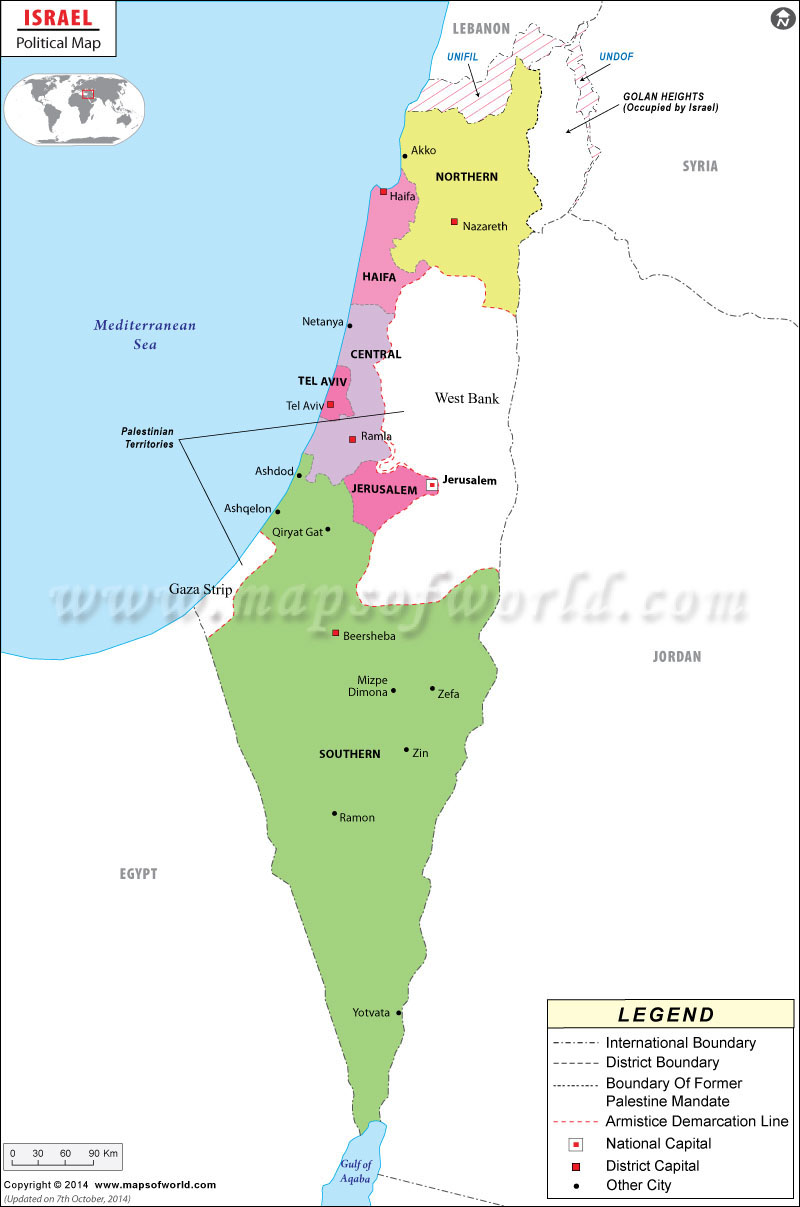
\includegraphics[height=7.5in]{israel-political-map}\\[\bigskipamount]
	\end{center}
}

\begin{document}
\maketitle
%%%%%%%%%%%%%%%%%%%%%%%%%%%%%%%%%%%%%%%%%%%%%%%%%%%%%%%%%%%%%%%%%%%%%%%%%%%%%%%
% Use different margins for the rest of the document
\newgeometry{margin = 0.75in}

%%%%%%%%%%%%%%%%%%%%%%%%%%%%%%%%%%%%%%%%%%%%%%%%%%%%%%%%%%%%%%%%%%%%%%%%%%%%%%%
%%%%%%%%%%%%%%%%%%%%%%%%%%%%%%%%%%%%%%%%%%%%%%%%%%%%%%%%%%%%%%%%%%%%%%%%%%%%%%%
\chapter{In Preparation}
%%%%%%%%%%%%%%%%%%%%%%%%%%%%%%%%%%%%%%%%%%%%%%%%%%%%%%%%%%%%%%%%%%%%%%%%%%%%%%%

\section{Preparation of This Document}
I wanted to do some deliberate preparation and pre-reading for the trip,
and typing it all out seemed like a good way to get that done.

\subsection{Fr. Gregory's Comments}
My Father-in-law was kind enough to send out some initial tips and thoughts
in several e-mails which  I consolidated here to form the framework of this 
document.

I left his notes intact here with only some grammatical enhancements and
embedding of the links to make it read a little nicer,
but otherwise it still reads as though he wrote it himself.

\subsection{Bible Verses}
The bible verses were copy-pasted from the website \url{https://www.biblegateway.com/}.

I selected the RSV translation since that seems to be the de-facto standard
for liturgical use, and I've had no major issues with the translation myself.

Using the website, it was really easy to just type in some verses and their
range, for example:
\href{https://www.biblegateway.com/passage/?search=Matthew+2%3A13-23&version=RSV}{
Matthew 2:13-23}

\subsection{Additional Contemplation}
I also wanted to have a paragraph of historical context about what we would be
seeing on the trip,
so I included what seemed most relevant

\subsection{Journaling}
I left extra space for writing notes and thoughts for the day as they occurred 
to me,
as well as set the expectation that Tatiana and I would try to write down a
journal entry at the end of each day, so that we could re-read it at some 
point in the future and remember some forgotten detail or significant impact
that gets too easily forgotten in the waves of reality that will inevitably
ensue.

\section{Preparations}
Before we left, Tatiana and I had a long checklist
of things that we needed to get done.

This included:
\begin{itemize}
    \item Getting our wills in order and ensuring our children and legacy would
    be cared for without causing undue burden on their guardians.
    \item Arranging for my mother to come and care for our children / animals / house while we are away.  This included:
    \begin{itemize}
        \item Buying a burner phone for my mom so she had emergency contact 
        capabilities (beyond using Google hangouts / skype for calling to
        Canada to keep in touch and for us to call back to her).
        \item Ensuring that she would be covered by our vehicle insurance
        \item Getting her on the phone list for school so she could know if 
        there was going to be cancellations
        (There's been at least 5 late-starts or total cancellations already 
        this year. Lots of snowfall in the 2016-2017 winter season)
        \item Having here come down early so that we can help show her our routine for the kids and where everything is.
        \item Providing her with emergency numbers for anything and everything.
    \end{itemize}
    \item Purchasing an international SIM card so that I can call/text while
    there for emergencies,
    as well as for uploading pictures and journaling
    directly to the cloud.
\end{itemize}

%%%%%%%%%%%%%%%%%%%%%%%%%%%%%%%%%%%%%%%%%%%%%%%%%%%%%%%%%%%%%%%%%%%%%%%%%%%%%%%
%%%%%%%%%%%%%%%%%%%%%%%%%%%%%%%%%%%%%%%%%%%%%%%%%%%%%%%%%%%%%%%%%%%%%%%%%%%%%%%
\chapter{The Journey}
%%%%%%%%%%%%%%%%%%%%%%%%%%%%%%%%%%%%%%%%%%%%%%%%%%%%%%%%%%%%%%%%%%%%%%%%%%%%%%%
\section{Jan 24 - Tuesday - Arrival Day}
Arrive in Tel Aviv and travel to and Check-in at Bethlehem

\subsection{Agenda}
\begin{description}
  \item[] Arrive Ben Gurion Airport Transfer to Bethlehem
  \item[Hotel] Dinner \& overnight in Bethlehem at the
    \href{http://www.grandpark.com/bethlehem/}{Grand Park Hotel}
\end{description}

\subsection{Notes from Fr. Gregory}
We will arrive in the late afternoon at Ben Gurion Airport in Tel Aviv.
By the time we clear customs, we will be quite tired and ready to transfer by bus 
to our hotel in Bethlehem.
(Originally this was the Grand Park Hotel, but I can't recall if our tour 
director told me that this had to be changed.
I am forwarding this to him as well for final clarification).


We will have dinner and rest at the hotel in Bethlehem in preparation for our
big first day.

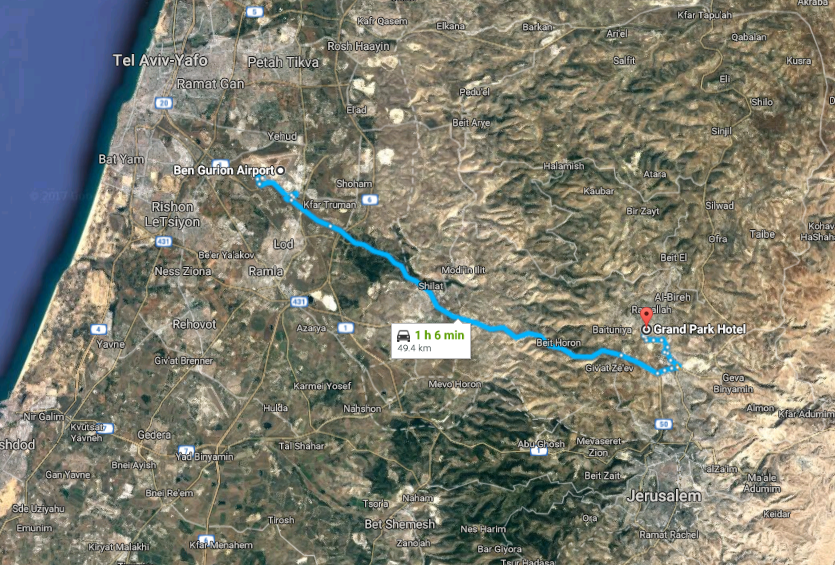
\includegraphics[width=\textwidth]{AirportToHotel}

\clearpage
\subsection{Daily Notes}
\clearpage
\subsection{Journal Entry}

%%%%%%%%%%%%%%%%%%%%%%%%%%%%%%%%%%%%%%%%%%%%%%%%%%%%%%%%%%%%%%%%%%%%%%%%%%%%%%%
\clearpage
\section{Jan 25 - Wednesday - Day 1}
Feast of St. Gregory the Theologian

\subsection{Agenda}
\begin{description}
	\item[08:00am] Bethlehem: Manger Square
	    \subitem Basilica \& Grotto of the Nativity
	    \subitem St. Jerome's Caves – Grotto of the Holy Innocent
	\item[09:00 or 10:00] Liturgy in the Church of the Nativity or in the 
		Fields of the Shepherds
		\subitem Beit Sahour: Shepherds’ Fields
	\item[Lunch] in Beit Sahour at the Shepherds’ Valley Restaurant 
	\item[Afternoon] Monastery of St. Sabbas in the desert 
	    (taxis to the monastery)
	    \subitem Shopping opportunity at an olive wood shop Dinner 
	    
	\item[Hotel] overnight in Bethlehem at the
	  \href{http://www.grandpark.com/bethlehem/}{Grand Park Hotel}
\end{description}

\subsection{Notes from Fr. Gregory}
We may be able to celebrate Liturgy this day. We shall see if this is possible. Either way, we will visit: the Church of the Nativity with Grotto beneath (spot where Christ was born); Grotto of the Holy Innocents; Shepherds' Fields (Ancient Byzantine Church remnant)...the Gospel passages for these sites are: 
Matthew 1:18-25; Matthew 2:1-12; Matthew 2:13-23; Luke 2:1-20

You may also study a bit more about the Holy Innocents on the
\href{https://oca.org/saints/lives/2007/12/29/103682-14000-infants-the-holy-innocents-slain-by-herod-at-bethlehem}{
    OCA website - Holy Innocents Slain By Herod at Bethlehem}. 

After lunch (remember, you have paid for three meals each day),
we will take taxis to St. Sabbas Monastery in the desert.
While women are not permitted in the monastery,
special provisions are made for them to be able to see down into the courtyard 
and (the last time I was here),
to venerate the Holy Relics. You can learn more about the monastery at
\href{http://stsabbas.org/jerusalem.html}{stsabbas.org}\footnote{If you poke 
    around on this site,
    you will find some important visitor etiquette that will 
    be beneficial for all of the Orthodox monasteries}
or at the \href{https://en.wikipedia.org/wiki/Mar_Saba}{
    Wikipedia page for Mar Saba}.

Read more about the 
\href{https://oca.org/saints/lives/2008/12/05/103477-venerable-sava-the-sanctified}{
	The Life of St. Sabbas} before we arrive.

We will then return to the hotel in Bethlehem for dinner and rest...

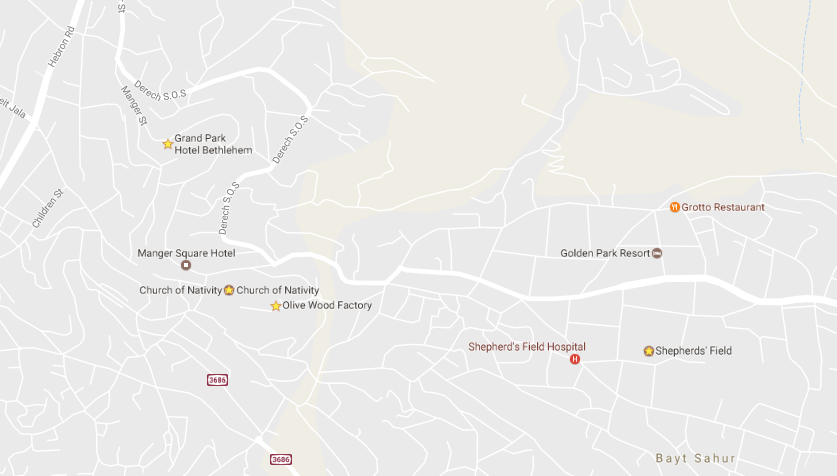
\includegraphics[width=\textwidth]{BethlehemSites}

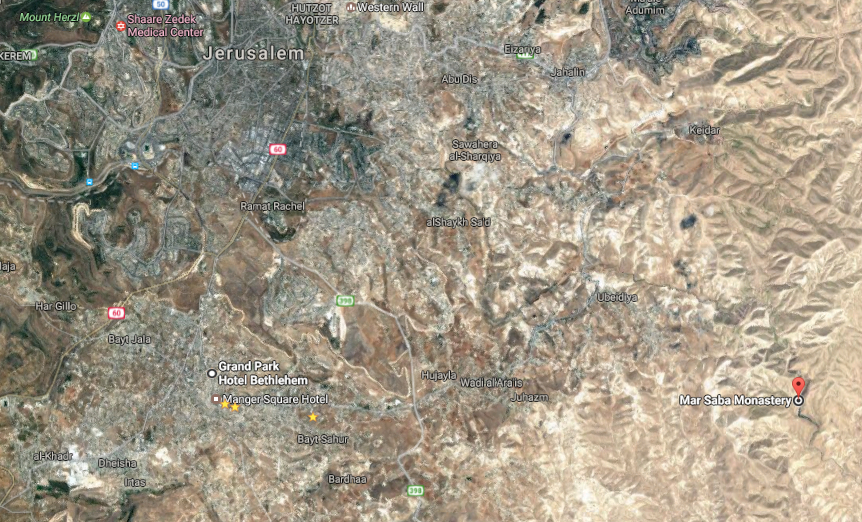
\includegraphics[width=\textwidth]{MarSabaMonastery}

\clearpage
\subsection{Church of the Nativity}
\begin{multicols}{2}

\subsubsection{\href{https://en.wikipedia.org/wiki/Church_of_the_Nativity}{
Church of the Nativity - Wikipedia}}

The Church of the Nativity is a basilica located in Bethlehem, West Bank.

The church was originally commissioned in 327 by Constantine the Great and his 
mother Helena over the site that was traditionally considered to be located 
over the cave that marks the birthplace of Jesus.
The Church of the Nativity site's original basilica was completed in 339 and 
destroyed by fire during the Samaritan Revolts in the 6\textsuperscript{th} 
century.
A new basilica was built 565 by Justinian, the Byzantine Emperor,
restoring the architectural tone of the original.
The site of the Church of the Nativity has had numerous additions since this 
second construction, including its prominent bell towers.
Due to its cultural and geographical history,
the site holds a prominent religious significance to those of the Christian 
faith.

The site of the Church of the Nativity is a World Heritage Site,
and was the first to be listed under Palestine by the United Nations 
Educational,
Scientific and Cultural Organization (UNESCO).
The site is also on UNESCO's List of World Heritage in Danger.

\begin{figure}[H]
\centering
\label{fig:GrottoOfTheNativity}
\caption{Grotto Of The Nativity}
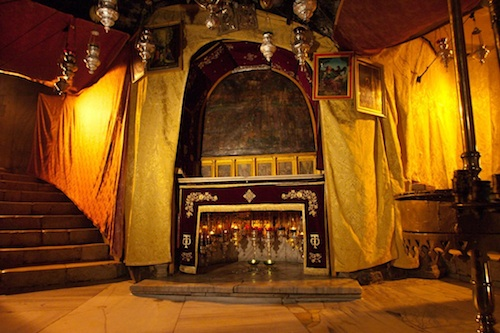
\includegraphics[width=\columnwidth]{GrottoOfTheNativity}
\end{figure}

\subsubsection{\href{http://www.bethlehem.custodia.org/default.asp?id=469}{
Church of the Nativity - bethlehem.custodia.org}}

The entrance today is placed sideways with respect to the location where Jesus was born, but it is thought that in the fourth century the entrance was located behind the presbytery. The small façades of the two side entrances date back to the times of the Crusaders.
The Grotto is entered by descending the stairs to the right of the iconostasis. Here the space is very narrow and restricted and the walls, which were originally irregular, form an almost-rectangular perimeter. The natural walls of the cave, decorated in the Constantine period, were covered with marble during the Byzantine period.
The Altar of the Nativity only began to be venerated in the Byzantine period when this space was created to commemorate the precise place in which Jesus had been born.
The current structure has been totally modified from that which was described by the pilgrim John Phocas and Abbot Daniel in the 12th century. Two red stone columns, and the inscription “Gloria in excelsis Deo et in terra pax hominibus”, overlook the altar, above which are representations of the Virgin and the Child in swaddling clothes, the scene of the washing, and that of the coming of the shepherds.
Beneath the altar is a star with the inscription “Hic de Virgine Maria Iesus Christus natus est” in memory of the precise spot of the Nativity. To the right of the altar is the place where Mary laid Jesus in the manger, also known as the Crib. At this point in the Grotto the floor is lower and the space is made up of columns similar to the Byzantine ones in the nave of the church, and by the remains of two Crusader columns.
In front of the Crib is a small altar dedicated to the Magi, where the Latins celebrate Holy Mass. The structure of the Crib is not the original one but is the result of alterations necessitated by the continuous wear and tear of time and the passage of pilgrims.
Following the fire of 1869 the walls of the Grotto were covered with asbestos to prevent further fires, a donation from the President of the French Republic Marshal Mac-Mahon in 1874. Below this covering the original Crusader marble is still visible, while above it can be seen wood panel paintings of limited artistic value.

\end{multicols}

\subsubsection{Scripture}

{\centering
\emph{\bibleverse{Matthew}(1:18-25) The Birth of Jesus the Messiah}\\
}
\begin{multicols}{2}
\vs{18}Now the birth of Jesus Christ took place in this way.
When his mother Mary had been betrothed to Joseph,
before they came together she was found to be with child of the Holy Spirit;
\vs{19}and her husband Joseph,
being a just man and unwilling to put her to shame,
resolved to divorce her quietly.
\vs{20}But as he considered this,
behold, an angel of the Lord appeared to him in a dream, saying,
``Joseph, son of David, do not fear to take Mary your wife,
for that which is conceived in her is of the Holy Spirit;
\vs{21}she will bear a son, and you shall call his name Jesus,
for he will save his people from their sins.''

\vs{22}All this took place to fulfill what the Lord had spoken by the prophet:

\begin{verse}
\vs{23}``Behold, a virgin shall conceive\\
and bear a son,\\
and his name shall be called Emman′u-el''\\
(which means, God with us).\\
\end{verse}

\vs{24}When Joseph woke from sleep,
he did as the angel of the Lord commanded him;
he took his wife,
\vs{25}but knew her not until she had borne a son;
and he called his name Jesus.
\end{multicols}

{\centering
\emph{\bibleverse{Matthew}(2:1-12) The Visit of the Wise Men}\\
}
\begin{multicols}{2}
\vs{1}Now when Jesus was born in Bethlehem of Judea in the days of Herod the king,
behold, wise men from the East came to Jerusalem, saying,
\vs{2}``Where is he who has been born king of the Jews?
For we have seen his star in the East, and have come to worship him.''
\vs{3}When Herod the king heard this, he was troubled, and all Jerusalem with him;
\vs{4}and assembling all the chief priests and scribes of the people,
he inquired of them where the Christ was to be born. \vs{5}They told him, ``In Bethlehem of Judea; for so it is written by the prophet:

\begin{verse}
\vs{6}`And you, O Bethlehem,\\
in the land of Judah,\\
are by no means least among the rulers of Judah;\\
for from you shall come a ruler\\
who will govern my people Israel.' ''\\ 
\end{verse}

\vs{7}Then Herod summoned the wise men secretly and ascertained from them what
time the star appeared;
\vs{8}and he sent them to Bethlehem, saying,
``Go and search diligently for the child,
and when you have found him bring me word,
that I too may come and worship him.''
\vs{9}When they had heard the king they went their way;
and lo, the star which they had seen in the East went before them,
till it came to rest over the place where the child was.
\vs{10}When they saw the star, they rejoiced exceedingly with great joy;
\vs{11} and going into the house they saw the child with Mary his mother,
and they fell down and worshiped him.
Then, opening their treasures, they offered him gifts,
gold and frankincense and myrrh.
\vs{12}And being warned in a dream not to return to Herod,
they departed to their own country by another way.
\end{multicols}

\subsection{Grotto of the Holy Innocents}
\begin{multicols}{2}

\subsubsection{\href{http://www.bethlehem.custodia.org/default.asp?id=473}{
Holy Innocents - bethlehem.custodia.org}}

With our back to the Altar of St. Joseph,
to our right is the Grotto of the Innocents in which one can see three 
arcosolium (or “bench”) type tombs,
each containing from two to five sepulchers.

Here the Massacre of the Innocents ordered by Herod the Great shortly after 
Jesus’ birth is commemorated.
In the first centuries, the memory of the Innocents was commemorated in an
adjoining cave,
which one can assume was a common grave in which numerous bones of corpses had 
been found.

\begin{figure}[H]
\centering
\label{fig:GrottoOfTheInnocents}
\caption{Grotto Of The Holy Innocents}
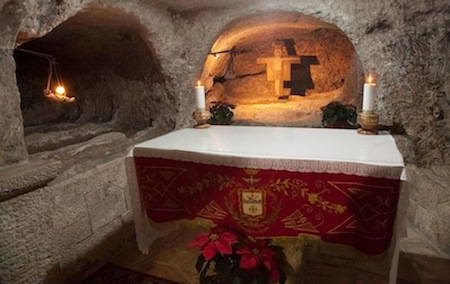
\includegraphics[width=\columnwidth]{GrottoOfTheInnocents}
\end{figure}

\end{multicols}

\subsubsection{Scripture}
{\centering
\emph{\bibleverse{Matthew}(2:13-23) The Escape to Egypt,
The Massacre of the Infants,
The Return from Egypt}\\
}
\begin{multicols}{2}
\vs{13}Now when they had departed, behold,
an angel of the Lord appeared to Joseph in a dream and said, ``Rise,
take the child and his mother, and flee to Egypt,
and remain there till I tell you; for Herod is about to search for the child,
to destroy him''
\vs{14}And he rose and took the child and his mother by night,
and departed to Egypt,
\vs{15}and remained there until the death of Herod.
This was to fulfill what the Lord had spoken by the prophet,
``Out of Egypt have I called my son.''

\vs{16}Then Herod, when he saw that he had been tricked by the wise men,
was in a furious rage,
and he sent and killed all the male children in Bethlehem and in all that 
region who were two years old or under,
according to the time which he had ascertained from the wise men.
\vs{17}Then was fulfilled what was spoken by the prophet Jeremiah:

\begin{verse}
\vs{18}``A voice was heard in Ramah,\\
wailing and loud lamentation,\\
Rachel weeping for her children;\\
she refused to be consoled,\\
because they were no more''\\
\end{verse}

\vs{19}But when Herod died, behold,
an angel of the Lord appeared in a dream to Joseph in Egypt, saying,
\vs{20}``Rise, take the child and his mother, and go to the land of Israel,
for those who sought the child’s life are dead.''
\vs{21}And he rose and took the child and his mother,
and went to the land of Israel.
\vs{22}But when he heard that Archela′us reigned over Judea in place of his 
father Herod, he was afraid to go there,
and being warned in a dream he withdrew to the district of Galilee.
\vs{23}And he went and dwelt in a city called Nazareth,
that what was spoken by the prophets might be fulfilled,
``He shall be called a Nazarene.''
\end{multicols}

\clearpage
\subsection{Shepherds' Fields}
\begin{multicols}{2}

\subsubsection{\href{http://www.custodia.org/default.asp?id=1888}{
Shepherds' Fields - Background}}

Some shepherds, amongst the most despised of the Jewish people,
went to adore Jesus. Dazzled by a great light,
an angel brought them the tidings of joy that the long-awaited Saviour had
been born.
And they heard a host of angels praising God who,
by sending the Messiah to the earth,
had shown His greatness to the celestial court and given salvation to men.

The Sanctuary, designed by Barluzzi, stands on a rock overlooking the ruins.
It has a dodecagonal shape with five apses having an inclined plane,
recalling the structure of a field tent like the one used by the shepherds at 
that time.
The light that penetrates the concrete and glass dome,
illuminating the interior calls to mind the divine light that appeared to the 
shepherds.

\begin{figure}[H]
\centering
\label{fig:ChurchOfTheAngelsAtShepherdsFields}
\caption{The Church of the Angels at Shepherd's Fields}
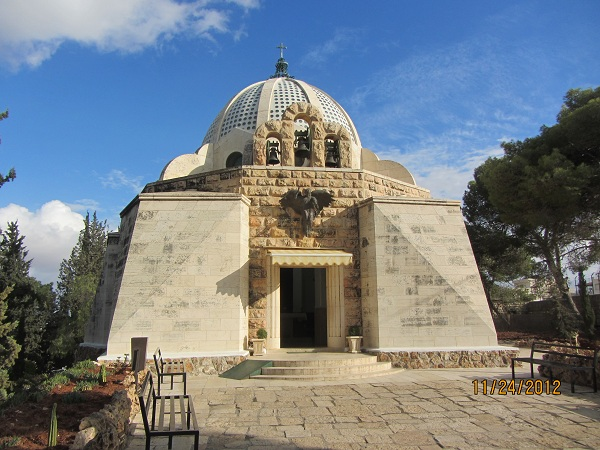
\includegraphics[width=\columnwidth]{ChurchOfTheAngelsAtShepherdsFields}
\end{figure}

\end{multicols}

\subsubsection{Scripture}
{\centering
\emph{\bibleverse{Luke}(2:1-20) The birth of Jesus,
	The Shepherds and the Angels}\\
}
\begin{multicols}{2}
\vs{1}In those days a decree went out from Caesar Augustus that all the world
should be enrolled.
\vs{2}This was the first enrollment, when Quirin′i-us was governor of Syria.
\vs{3}And all went to be enrolled, each to his own city.
\vs{4}And Joseph also went up from Galilee, from the city of Nazareth,
to Judea, to the city of David, which is called Bethlehem,
because he was of the house and lineage of David,
\vs{5}to be enrolled with Mary, his betrothed, who was with child.
\vs{6}And while they were there, the time came for her to be delivered.
\vs{7}And she gave birth to her first-born son and wrapped him in swaddling
cloths, and laid him in a manger,
because there was no place for them in the inn.

\vs{8} And in that region there were shepherds out in the field,
keeping watch over their flock by night.
\vs{9}And an angel of the Lord appeared to them,
and the glory of the Lord shone around them,
and they were filled with fear.
\vs{10}And the angel said to them, ``Be not afraid; for behold,
I bring you good news of a great joy which will come to all the people;
\vs{11}for to you is born this day in the city of David a Savior,
who is Christ the Lord.
\vs{12}And this will be a sign for you:
you will find a babe wrapped in swaddling cloths and lying in a manger.''
\vs{13}And suddenly there was with the angel a multitude of the heavenly host 
praising God and saying,

\begin{verse}
\vs{14}``Glory to God in the highest,\\
and on earth peace among men with whom he is pleased!''\\
\end{verse}

\vs{15}When the angels went away from them into heaven,
the shepherds said to one another,
``Let us go over to Bethlehem and see this thing that has happened,
which the Lord has made known to us.''
\vs{16}And they went with haste, and found Mary and Joseph,
and the babe lying in a manger.
\vs{17}And when they saw it they made known the saying which had been told
them concerning this child;
\vs{18}and all who heard it wondered at what the shepherds told them.
\vs{19}But Mary kept all these things, pondering them in her heart.
\vs{20}And the shepherds returned,
glorifying and praising God for all they had heard and seen,
as it had been told them.
\end{multicols}

\clearpage
\subsection{Daily Notes}

\clearpage
\subsection{Journal Entry}

%%%%%%%%%%%%%%%%%%%%%%%%%%%%%%%%%%%%%%%%%%%%%%%%%%%%%%%%%%%%%%%%%%%%%%%%%%%%%%%
\clearpage
\section{Jan 26 - Thursday - Day 2}
Jerusalem
\subsection{Agenda}
\begin{description}
	\item[08:00] Check-out of the hotel – Drive to Jerusalem (east first)
	    \subitem Mount of Olives: Russian Orthodox Monastery
	    \subitem Pater Noster Church -- Panoramic view
	    \subitem Palm Sunday route
	    \subitem Dominus Flevit Chapel
	    \subitem St. Mary Magdalene Russian Orthodox Church
	        (open 10:00 – 12:00)
	    \subitem Garden of Gethsemane
	    \subitem Church of All Nations (if time permits)
	    \subitem Tomb of the Virgin Mary
	\item[Lunch] in Jerusalem at the
			St. Andrew’s Guest House or Notre Dame Center
	\item[Afternoon] West Jerusalem
	    \subitem Greek Orthodox Monastery of the Holy Cross (10:00 – 16:00)
		\subitem Village of Ein Karem: Church of John the Baptist 
		\subitem Israel Museum: Model of Ancient Jerusalem
		\subitem Shrine of the Book (optional)
	\item[Hotel] Dinner \& overnight in Jerusalem at the
	    \href{http://goldenwalls.com/}{Golden Walls Hotel}
\end{description}

\subsection{Notes from Fr. Gregory}
We will have breakfast at the hotel and then take all of our luggage with us 
as we check out of the first hotel.
Today we drive to Jerusalem, which is not that far away from Bethlehem.
This morning we will be in the area of the Mount of Olives and the Garden of
Gethsemane.
Our sites will include several Russian Orthodox monasteries;
one on the Mount of Olives and one at Gethsemane,
the Tomb of the Holy Mother of God,
and perhaps the Chapel of the Ascension.
All of the sites on this day are outside of the walls of the Old City and we
will have beautiful views of Jerusalem from these heights.

For the Mount of Olives, the Epistle and Gospel passages to be read are from
the Ascension (Acts of the Apostles 1:1-12 and Luke 24:36-53).
Here is a good site for the 
\href{http://www.sacred-destinations.com/israel/jerusalem-chapel-of-ascension}{
    Chapel of the Ascension}.

St. Pelagia the Penitent's Tomb is also here...we will need to ask the guard 
at the Chapel of the Ascension if we wish to see and venerate it...
\href{http://www.antiochian.org/node/16762}{
	Her life is here}

Here is 
\href{http://www.pravoslavie.ru/english/46854.htm}{
	a very interesting site highlighting the history of the Mount of Olives},
 including the present day Russian Mission located there.
 This includes the Chapel of St. John the Baptist,
 built over the site where his honorable head was discovered.

And here is \href{http://jerusalem-mission.org/convent_ascension.html}{
	a history of the Russian Convent on the Mount of Olives}.

In this area are also the Dominus Flevit (The Lord Wept) Chapel,
Church of the Pater Noster (Our Father) and the Church of All Nations.
You may look those up as well and we will try to visit them if we have the 
time.

In general, the scriptures concerning Christ's Agony in the Garden of 
Gethsemane are Matthew 26:36-56; Mark 14:32-50; Luke 22:40-53; John 18:1-12.

We will also visit the Russian Orthodox Convent of St. Mary Magdalene in
Gethsemane.
\href{http://www.pravoslavie.ru/english/63239.htm}{
The relics of Grand Duchess Elizabeth and the Nun Barbara} are housed here.

Hopefully, the sisters can tell us a little about the traditional location of 
Christ's Weeping in the Garden and why the monastery was built here.

Finally, we cannot forget the Tomb of the Holy Mother of God;
it is also here, right next to the Church of All Nations.
\href{https://orthodoxword.wordpress.com/2010/08/15/the-tomb-of-the-most-holy-virgin-jerusalem/}{
Here is a site} highlighting that Holy Place.

I also wish to make it a point to visit the relatively new Greek Orthodox
Church of the Protomartyr Stephen,
built near the site of his traditional martyrdom by stoning;
the account of his martyrdom can be found in
Acts of the Apostles 6:8-7:5, 46-60.

After Lunch,
we will visit the Greek Orthodox Monastery of the Holy Cross
\href{http://www.biblewalks.com/Sites/CrossMonastery.html}{
	which you can visit here}.

We are also scheduled to visit the Village of Ein Karem (Gornya)
on this day;
specifically, the Greek Orthodox Church of St. John the Baptist;
\href{https://www.holyland-pilgrimage.org/ein-karem-home-of-john-the-baptist-and-place-of-the-visitation}{read about this village here}.

One other thought for this day...what a blessing to visit Katamon
(The Monastery of St. Simeon the God-Receiver);
we shall try to do our best to see these Holy Places given our time
restraints.
Read the story of St. Simeon the God-Receiver in the Holy Scriptures at
Luke 2:25-38.
\href{http://www.goisrael.com/Tourism_Eng/Tourist%20Information/Christian%20Themes/Details/Pages/St.%20Simeon%E2%80%99s%20Monastery%20chr.aspx}
	{Here is a short description of the site}.
	
I believe that we will stay at the Golden Walls Hotel in Jerusalem on this
night; so we will check in and have dinner there...
rest up because we have only toured for two days
(and just describing these two days has already made me tired)!!!

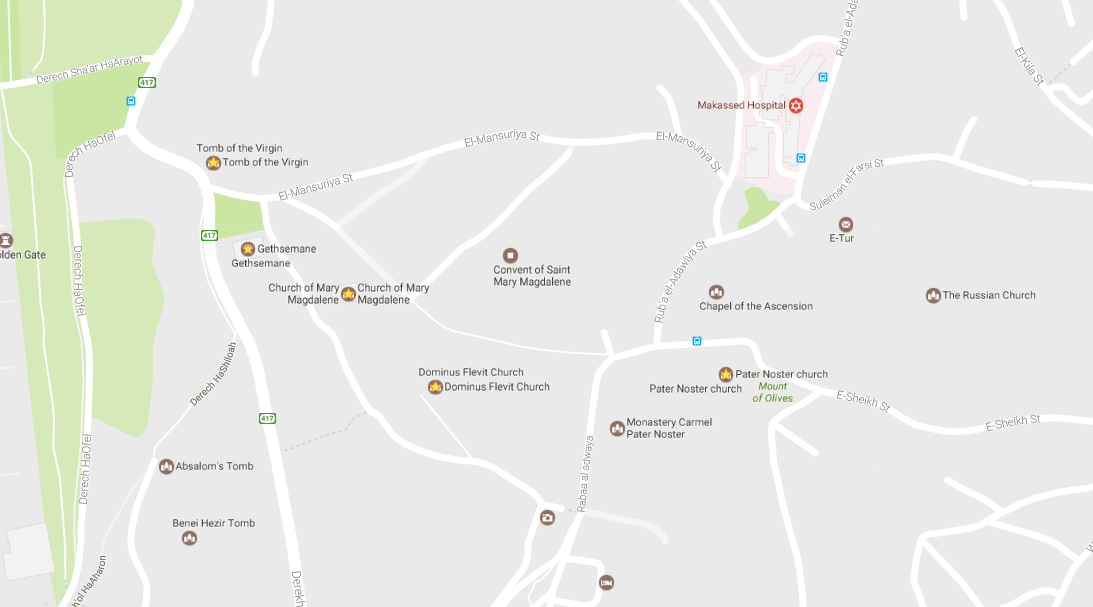
\includegraphics[width=\textwidth]{MountOfOlives}

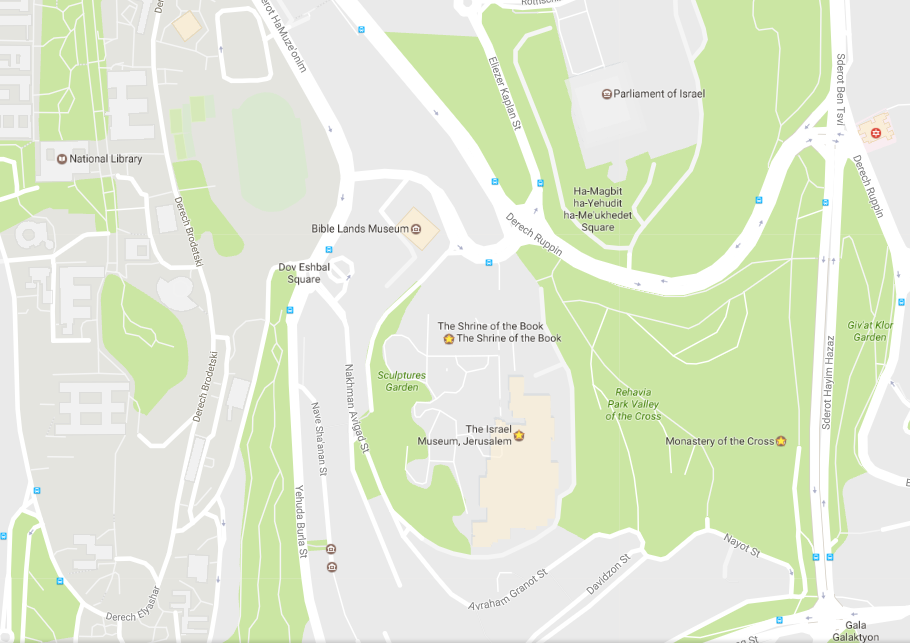
\includegraphics[width=\textwidth]{IsraelMuseum}

\clearpage
\subsection{Mount of Olives}
\begin{multicols}{2}
	\mbox{}
\end{multicols}
\subsubsection{Scripture}

{\centering
	\emph{\bibleverse{Acts}(1:1-12) The Promise of the Holy Spirit, The Ascension of Jesus, Matthias Chosen to Replace Judas}\\
}
\begin{multicols}{2}

In the first book, O The-oph′ilus, I have dealt with all that Jesus began to do and teach, 2 until the day when he was taken up, after he had given commandment through the Holy Spirit to the apostles whom he had chosen. 3 To them he presented himself alive after his passion by many proofs, appearing to them during forty days, and speaking of the kingdom of God. 4 And while staying[a] with them he charged them not to depart from Jerusalem, but to wait for the promise of the Father, which, he said, “you heard from me, 5 for John baptized with water, but before many days you shall be baptized with the Holy Spirit.”

6 So when they had come together, they asked him, “Lord, will you at this time restore the kingdom to Israel?” 7 He said to them, “It is not for you to know times or seasons which the Father has fixed by his own authority. 8 But you shall receive power when the Holy Spirit has come upon you; and you shall be my witnesses in Jerusalem and in all Judea and Samar′ia and to the end of the earth.” 9 And when he had said this, as they were looking on, he was lifted up, and a cloud took him out of their sight. 10 And while they were gazing into heaven as he went, behold, two men stood by them in white robes, 11 and said, “Men of Galilee, why do you stand looking into heaven? This Jesus, who was taken up from you into heaven, will come in the same way as you saw him go into heaven.”

12 Then they returned to Jerusalem from the mount called Olivet, which is near Jerusalem, a sabbath day’s journey away
\end{multicols}

{\centering
	\emph{\bibleverse{Luke}(24:36-53) Jesus Appears to His Disciples, The Ascension of Jesus}\\
}
\begin{multicols}{2}
36 As they were saying this, Jesus himself stood among them. 37 But they were startled and frightened, and supposed that they saw a spirit. 38 And he said to them, “Why are you troubled, and why do questionings rise in your hearts? 39 See my hands and my feet, that it is I myself; handle me, and see; for a spirit has not flesh and bones as you see that I have.” 41 And while they still disbelieved for joy, and wondered, he said to them, “Have you anything here to eat?” 42 They gave him a piece of broiled fish, 43 and he took it and ate before them.

44 Then he said to them, “These are my words which I spoke to you, while I was still with you, that everything written about me in the law of Moses and the prophets and the psalms must be fulfilled.” 45 Then he opened their minds to understand the scriptures, 46 and said to them, “Thus it is written, that the Christ should suffer and on the third day rise from the dead, 47 and that repentance and forgiveness of sins should be preached in his name to all nations, beginning from Jerusalem. 48 You are witnesses of these things. 49 And behold, I send the promise of my Father upon you; but stay in the city, until you are clothed with power from on high.”

50 Then he led them out as far as Bethany, and lifting up his hands he blessed them. 51 While he blessed them, he parted from them, and was carried up into heaven. 52 And they[e] returned to Jerusalem with great joy, 53 and were continually in the temple blessing God.

\end{multicols}

\clearpage
\subsection{Gethsemane}
\begin{multicols}{2}
	\mbox{}
\end{multicols}
\subsubsection{Scripture}

{\centering
	\emph{\bibleverse{Matthew}(26:36-56) Jesus Prays in Gethsemane, The Betrayal and Arrest of Jesus}\\
}
\begin{multicols}{2}
36 Then Jesus went with them to a place called Gethsem′ane, and he said to his disciples, “Sit here, while I go yonder and pray.” 37 And taking with him Peter and the two sons of Zeb′edee, he began to be sorrowful and troubled. 38 Then he said to them, “My soul is very sorrowful, even to death; remain here, and watch with me.” 39 And going a little farther he fell on his face and prayed, “My Father, if it be possible, let this cup pass from me; nevertheless, not as I will, but as thou wilt.” 40 And he came to the disciples and found them sleeping; and he said to Peter, “So, could you not watch with me one hour? 41 Watch and pray that you may not enter into temptation; the spirit indeed is willing, but the flesh is weak.” 42 Again, for the second time, he went away and prayed, “My Father, if this cannot pass unless I drink it, thy will be done.” 43 And again he came and found them sleeping, for their eyes were heavy. 44 So, leaving them again, he went away and prayed for the third time, saying the same words. 45 Then he came to the disciples and said to them, “Are you still sleeping and taking your rest? Behold, the hour is at hand, and the Son of man is betrayed into the hands of sinners. 46 Rise, let us be going; see, my betrayer is at hand.”

47 While he was still speaking, Judas came, one of the twelve, and with him a great crowd with swords and clubs, from the chief priests and the elders of the people. 48 Now the betrayer had given them a sign, saying, “The one I shall kiss is the man; seize him.” 49 And he came up to Jesus at once and said, “Hail, Master!” And he kissed him. 50 Jesus said to him, “Friend, why are you here?” Then they came up and laid hands on Jesus and seized him. 51 And behold, one of those who were with Jesus stretched out his hand and drew his sword, and struck the slave of the high priest, and cut off his ear. 52 Then Jesus said to him, “Put your sword back into its place; for all who take the sword will perish by the sword. 53 Do you think that I cannot appeal to my Father, and he will at once send me more than twelve legions of angels? 54 But how then should the scriptures be fulfilled, that it must be so?” 55 At that hour Jesus said to the crowds, “Have you come out as against a robber, with swords and clubs to capture me? Day after day I sat in the temple teaching, and you did not seize me. 56 But all this has taken place, that the scriptures of the prophets might be fulfilled.” Then all the disciples forsook him and fled.
\end{multicols}

{\centering
	\emph{\bibleverse{Mark}(14:32-50) Jesus Prays in Gethsemane, The Betrayal and Arrest of Jesus}\\
}
\begin{multicols}{2}
32 And they went to a place which was called Gethsem′ane; and he said to his disciples, “Sit here, while I pray.” 33 And he took with him Peter and James and John, and began to be greatly distressed and troubled. 34 And he said to them, “My soul is very sorrowful, even to death; remain here, and watch.” 35 And going a little farther, he fell on the ground and prayed that, if it were possible, the hour might pass from him. 36 And he said, “Abba, Father, all things are possible to thee; remove this cup from me; yet not what I will, but what thou wilt.” 37 And he came and found them sleeping, and he said to Peter, “Simon, are you asleep? Could you not watch one hour? 38 Watch and pray that you may not enter into temptation; the spirit indeed is willing, but the flesh is weak.” 39 And again he went away and prayed, saying the same words. 40 And again he came and found them sleeping, for their eyes were very heavy; and they did not know what to answer him. 41 And he came the third time, and said to them, “Are you still sleeping and taking your rest? It is enough; the hour has come; the Son of man is betrayed into the hands of sinners. 42 Rise, let us be going; see, my betrayer is at hand.”

43 And immediately, while he was still speaking, Judas came, one of the twelve, and with him a crowd with swords and clubs, from the chief priests and the scribes and the elders. 44 Now the betrayer had given them a sign, saying, “The one I shall kiss is the man; seize him and lead him away under guard.” 45 And when he came, he went up to him at once, and said, “Master!” And he kissed him. 46 And they laid hands on him and seized him. 47 But one of those who stood by drew his sword, and struck the slave of the high priest and cut off his ear. 48 And Jesus said to them, “Have you come out as against a robber, with swords and clubs to capture me? 49 Day after day I was with you in the temple teaching, and you did not seize me. But let the scriptures be fulfilled.” 50 And they all forsook him, and fled.
\end{multicols}

{\centering
	\emph{\bibleverse{Luke}(22:40-53) Jesus Prays in Gethsemane, The Betrayal and Arrest of Jesus}\\
}
\begin{multicols}{2}
40 And when he came to the place he said to them, “Pray that you may not enter into temptation.” 41 And he withdrew from them about a stone’s throw, and knelt down and prayed, 42 “Father, if thou art willing, remove this cup from me; nevertheless not my will, but thine, be done.” 45 And when he rose from prayer, he came to the disciples and found them sleeping for sorrow, 46 and he said to them, “Why do you sleep? Rise and pray that you may not enter into temptation.”

47 While he was still speaking, there came a crowd, and the man called Judas, one of the twelve, was leading them. He drew near to Jesus to kiss him; 48 but Jesus said to him, “Judas, would you betray the Son of man with a kiss?” 49 And when those who were about him saw what would follow, they said, “Lord, shall we strike with the sword?” 50 And one of them struck the slave of the high priest and cut off his right ear. 51 But Jesus said, “No more of this!” And he touched his ear and healed him. 52 Then Jesus said to the chief priests and officers of the temple and elders, who had come out against him, “Have you come out as against a robber, with swords and clubs? 53 When I was with you day after day in the temple, you did not lay hands on me. But this is your hour, and the power of darkness.”
\end{multicols}

{\centering
	\emph{\bibleverse{John}(18:1-12) The Betrayal and Arrest of Jesus, Jesus before the High Priest}\\
}
\begin{multicols}{2}
	When Jesus had spoken these words, he went forth with his disciples across the Kidron valley, where there was a garden, which he and his disciples entered. 2 Now Judas, who betrayed him, also knew the place; for Jesus often met there with his disciples. 3 So Judas, procuring a band of soldiers and some officers from the chief priests and the Pharisees, went there with lanterns and torches and weapons. 4 Then Jesus, knowing all that was to befall him, came forward and said to them, “Whom do you seek?” 5 They answered him, “Jesus of Nazareth.” Jesus said to them, “I am he.” Judas, who betrayed him, was standing with them. 6 When he said to them, “I am he,” they drew back and fell to the ground. 7 Again he asked them, “Whom do you seek?” And they said, “Jesus of Nazareth.” 8 Jesus answered, “I told you that I am he; so, if you seek me, let these men go.” 9 This was to fulfil the word which he had spoken, “Of those whom thou gavest me I lost not one.” 10 Then Simon Peter, having a sword, drew it and struck the high priest’s slave and cut off his right ear. The slave’s name was Malchus. 11 Jesus said to Peter, “Put your sword into its sheath; shall I not drink the cup which the Father has given me?”
	
	 So the band of soldiers and their captain and the officers of the Jews seized Jesus and bound him.
\end{multicols}

\clearpage
\subsection{Greek Orthodox Church of the Protomartyr Stephen}
\begin{multicols}{2}
	\mbox{}
\end{multicols}
\subsubsection{Scripture}

{\centering
	\emph{\bibleverse{Acts}(6:8-7:60) The Arrest of Stephen,
		Stephen’s Speech to the Council,
		The Stoning of Stephen}\\
}
\begin{multicols}{2}
8 And Stephen, full of grace and power, did great wonders and signs among the people. 9 Then some of those who belonged to the synagogue of the Freedmen (as it was called), and of the Cyre′nians, and of the Alexandrians, and of those from Cili′cia and Asia, arose and disputed with Stephen. 10 But they could not withstand the wisdom and the Spirit with which he spoke. 11 Then they secretly instigated men, who said, “We have heard him speak blasphemous words against Moses and God.” 12 And they stirred up the people and the elders and the scribes, and they came upon him and seized him and brought him before the council, 13 and set up false witnesses who said, “This man never ceases to speak words against this holy place and the law; 14 for we have heard him say that this Jesus of Nazareth will destroy this place, and will change the customs which Moses delivered to us.” 15 And gazing at him, all who sat in the council saw that his face was like the face of an angel.

7 And the high priest said, “Is this so?” 2 And Stephen said:

“Brethren and fathers, hear me. The God of glory appeared to our father Abraham, when he was in Mesopota′mia, before he lived in Haran, 3 and said to him, ‘Depart from your land and from your kindred and go into the land which I will show you.’ 4 Then he departed from the land of the Chalde′ans, and lived in Haran. And after his father died, God removed him from there into this land in which you are now living; 5 yet he gave him no inheritance in it, not even a foot’s length, but promised to give it to him in possession and to his posterity after him, though he had no child. 6 And God spoke to this effect, that his posterity would be aliens in a land belonging to others, who would enslave them and ill-treat them four hundred years. 7 ‘But I will judge the nation which they serve,’ said God, ‘and after that they shall come out and worship me in this place.’ 8 And he gave him the covenant of circumcision. And so Abraham became the father of Isaac, and circumcised him on the eighth day; and Isaac became the father of Jacob, and Jacob of the twelve patriarchs.

9 “And the patriarchs, jealous of Joseph, sold him into Egypt; but God was with him, 10 and rescued him out of all his afflictions, and gave him favor and wisdom before Pharaoh, king of Egypt, who made him governor over Egypt and over all his household. 11 Now there came a famine throughout all Egypt and Canaan, and great affliction, and our fathers could find no food. 12 But when Jacob heard that there was grain in Egypt, he sent forth our fathers the first time. 13 And at the second visit Joseph made himself known to his brothers, and Joseph’s family became known to Pharaoh. 14 And Joseph sent and called to him Jacob his father and all his kindred, seventy-five souls; 15 and Jacob went down into Egypt. And he died, himself and our fathers, 16 and they were carried back to Shechem and laid in the tomb that Abraham had bought for a sum of silver from the sons of Hamor in Shechem.

17 “But as the time of the promise drew near, which God had granted to Abraham, the people grew and multiplied in Egypt 18 till there arose over Egypt another king who had not known Joseph. 19 He dealt craftily with our race and forced our fathers to expose their infants, that they might not be kept alive. 20 At this time Moses was born, and was beautiful before God. And he was brought up for three months in his father’s house; 21 and when he was exposed, Pharaoh’s daughter adopted him and brought him up as her own son. 22 And Moses was instructed in all the wisdom of the Egyptians, and he was mighty in his words and deeds.

23 “When he was forty years old, it came into his heart to visit his brethren, the sons of Israel. 24 And seeing one of them being wronged, he defended the oppressed man and avenged him by striking the Egyptian. 25 He supposed that his brethren understood that God was giving them deliverance by his hand, but they did not understand. 26 And on the following day he appeared to them as they were quarreling and would have reconciled them, saying, ‘Men, you are brethren, why do you wrong each other?’ 27 But the man who was wronging his neighbor thrust him aside, saying, ‘Who made you a ruler and a judge over us? 28 Do you want to kill me as you killed the Egyptian yesterday?’ 29 At this retort Moses fled, and became an exile in the land of Mid′ian, where he became the father of two sons.

30 “Now when forty years had passed, an angel appeared to him in the wilderness of Mount Sinai, in a flame of fire in a bush. 31 When Moses saw it he wondered at the sight; and as he drew near to look, the voice of the Lord came, 32 ‘I am the God of your fathers, the God of Abraham and of Isaac and of Jacob.’ And Moses trembled and did not dare to look. 33 And the Lord said to him, ‘Take off the shoes from your feet, for the place where you are standing is holy ground. 34 I have surely seen the ill-treatment of my people that are in Egypt and heard their groaning, and I have come down to deliver them. And now come, I will send you to Egypt.’

35 “This Moses whom they refused, saying, ‘Who made you a ruler and a judge?’ God sent as both ruler and deliverer by the hand of the angel that appeared to him in the bush. 36 He led them out, having performed wonders and signs in Egypt and at the Red Sea, and in the wilderness for forty years. 37 This is the Moses who said to the Israelites, ‘God will raise up for you a prophet from your brethren as he raised me up.’ 38 This is he who was in the congregation in the wilderness with the angel who spoke to him at Mount Sinai, and with our fathers; and he received living oracles to give to us. 39 Our fathers refused to obey him, but thrust him aside, and in their hearts they turned to Egypt, 40 saying to Aaron, ‘Make for us gods to go before us; as for this Moses who led us out from the land of Egypt, we do not know what has become of him.’ 41 And they made a calf in those days, and offered a sacrifice to the idol and rejoiced in the works of their hands. 42 But God turned and gave them over to worship the host of heaven, as it is written in the book of the prophets:

\begin{verse}
‘Did you offer to me slain beasts and sacrifices,\\
forty years in the wilderness, O house of Israel?\\
43 And you took up the tent of Moloch,\\
and the star of the god Rephan,\\
the figures which you made to worship;\\
and I will remove you beyond Babylon.’\\
\end{verse}

44 “Our fathers had the tent of witness in the wilderness, even as he who spoke to Moses directed him to make it, according to the pattern that he had seen. 45 Our fathers in turn brought it in with Joshua when they dispossessed the nations which God thrust out before our fathers. So it was until the days of David, 46 who found favor in the sight of God and asked leave to find a habitation for the God of Jacob. 47 But it was Solomon who built a house for him. 48 Yet the Most High does not dwell in houses made with hands; as the prophet says,

\begin{verse}
49 ‘Heaven is my throne,\\
and earth my footstool.\\
What house will you build for me, says the Lord,\\
or what is the place of my rest?\\
50 Did not my hand make all these things?’\\
\end{verse}
51 “You stiff-necked people, uncircumcised in heart and ears, you always resist the Holy Spirit. As your fathers did, so do you. 52 Which of the prophets did not your fathers persecute? And they killed those who announced beforehand the coming of the Righteous One, whom you have now betrayed and murdered, 53 you who received the law as delivered by angels and did not keep it.”

54 Now when they heard these things they were enraged, and they ground their teeth against him. 55 But he, full of the Holy Spirit, gazed into heaven and saw the glory of God, and Jesus standing at the right hand of God; 56 and he said, “Behold, I see the heavens opened, and the Son of man standing at the right hand of God.” 57 But they cried out with a loud voice and stopped their ears and rushed together upon him. 58 Then they cast him out of the city and stoned him; and the witnesses laid down their garments at the feet of a young man named Saul. 59 And as they were stoning Stephen, he prayed, “Lord Jesus, receive my spirit.” 60 And he knelt down and cried with a loud voice, “Lord, do not hold this sin against them.” And when he had said this, he fell asleep.
\end{multicols}

\clearpage
\subsection{Katamon -- The Monastery of St. Simeon the God-Receiver}
\begin{multicols}{2}
	\mbox{}
\end{multicols}
\subsubsection{Scripture}

{\centering
	\emph{\bibleverse{Luke}( 2:21-38 ) Jesus Is Named, Jesus Is Presented in the Temple}\\
}
\begin{multicols}{2}
21 And at the end of eight days, when he was circumcised, he was called Jesus, the name given by the angel before he was conceived in the womb.

22 And when the time came for their purification according to the law of Moses, they brought him up to Jerusalem to present him to the Lord 23 (as it is written in the law of the Lord, “Every male that opens the womb shall be called holy to the Lord”) 24 and to offer a sacrifice according to what is said in the law of the Lord, “a pair of turtledoves, or two young pigeons.” 25 Now there was a man in Jerusalem, whose name was Simeon, and this man was righteous and devout, looking for the consolation of Israel, and the Holy Spirit was upon him. 26 And it had been revealed to him by the Holy Spirit that he should not see death before he had seen the Lord’s Christ. 27 And inspired by the Spirit[a] he came into the temple; and when the parents brought in the child Jesus, to do for him according to the custom of the law, 28 he took him up in his arms and blessed God and said,

\begin{verse}
29 “Lord, now lettest thou thy servant depart in peace,\\
according to thy word;\\
30 for mine eyes have seen thy salvation\\
31 which thou hast prepared in the presence of all peoples,\\
32 a light for revelation to the Gentiles,\\
and for glory to thy people Israel.”\\
\end{verse}

33 And his father and his mother marveled at what was said about him; 34 and Simeon blessed them and said to Mary his mother,

\begin{verse}
“Behold, this child is set for the fall and rising of many in Israel,\\
and for a sign that is spoken against\\
35 (and a sword will pierce through your own soul also),\\
that thoughts out of many hearts may be revealed.”\\
\end{verse}

36 And there was a prophetess, Anna, the daughter of Phan′u-el, of the tribe of Asher; she was of a great age, having lived with her husband seven years from her virginity, 37 and as a widow till she was eighty-four. She did not depart from the temple, worshiping with fasting and prayer night and day. 38 And coming up at that very hour she gave thanks to God, and spoke of him to all who were looking for the redemption of Jerusalem.
\end{multicols}

\clearpage
\subsection{Daily Notes}

\clearpage
\subsection{Journal Entry}

%%%%%%%%%%%%%%%%%%%%%%%%%%%%%%%%%%%%%%%%%%%%%%%%%%%%%%%%%%%%%%%%%%%%%%%%%%%%%%%
\clearpage
\section{Jan 27 - Friday - Day 3}
Old Jerusalem
\subsection{Agenda}
\begin{description}
	\item[08:00am] Depart to  \href{http://jerusalem.com/map#!/explore/view}{
			Old City of Jerusalem (click for interactive map)}:
		\subitem Dung Gate – Western Wall
		\subitem Temple Mount:
		    view the El Aqsa Mosque \& the Dome of the Rock 
		\subitem Via Dolorosa:
		    Pool of Bethesda -- Church of St Anne
		\subitem Monastery of Sts. Joachim and Anna:
		    birthplace of the Mother of God.
	\item[Lunch] in the Armenian Quarter at the Bulghourji Restaurant 
	\item[Afternoon] Greek Orthodox Patriarchate (blessing by the Patriarch) 
		\subitem Church of the Holy Sepulchre
	\item[Hotel] Dinner \& overnight in Jerusalem at the
	  \href{http://goldenwalls.com/}{Golden Walls Hotel}
\end{description}

\subsection{Notes from Fr. Gregory}
On Day 3 we will enter the old city of Jerusalem through the Dung Gate.
We will go to the Temple Mount and see the Western Wall
(last remaining piece of the Old Temple)...as well as the Dome of the Rock.
It may be possible, while at the Temple Mount (Sion),
to visit the Upper Room and even King David's Tomb...
we will check on these sites when we get on the ground over there.
Holy Scripture: Mark 14:12-26; Matthew 26:17-30;
John 13:1-17 and (Pentecost) Acts 2:1-21.

Next we will be on the Via Dolorosa (Way of the Cross)...
this is the traditional path taken by Christ as He carried the Holy Cross to
Golgotha...
it includes the Lithostrotos (Flagellation Chapel) and 
\href{http://www.mikemasonbooks.com/the-lithostrotos-chapter-57-of-jesus-his-story-in-stone/}{
	a good explanation is here}.

In this vicinity is the Sheep's Pool (Bethesda)...
read the Gospel of John 5:1-15 and, while I am thinking of pools,
just outside of the Old City is Siloam...
read John 9:1-38. We shall try to get there as well.
Before getting to the Holy Sepulchre,
there remains the Church of St. Anne and the Monastery of Sts. Joachim and
Anna...\href{http://www.seetheholyland.net/church-of-st-anne/}{
	you can look here} for some background.
\href{http://www.johnsanidopoulos.com/2011/09/video-home-of-sts-joachim-and-anna-in.html}{
Also see this video, with Greek chanting.}

After lunch, we are scheduled to Greek Orthodox Patriarchate of Jerusalem and,
if the Lord blesses it, to receive the Blessing of the Patriarch of Jerusalem.
Following this, we will visit the holiest site in all of Christendom...
the Church of the Holy Sepulchre.
There is too much here to describe.
Here are SOME (not all) of the relevant Gospel passages covered beneath the 
roof of this incredible Holy Place:
Mark 15:43-47 (The Anointing Stone inside the entrance);
Matthew 27:27-56 (Golgotha...each evangelist has a passage announcing this); 
and the Life-Giving Tomb of Christ...
Mark 15:42-16:8
(each evangelist also joyously announces this reality as well).
\href{https://orthodoxwiki.org/Church_of_the_Holy_Sepulchre_(Jerusalem)}{
	Here is link that should give us a pretty good start}.

We then return for dinner and overnight to our hotel in Jerusalem.

\href{http://wikitravel.org/en/Jerusalem/Old_City}{
	The old city is divided into 4 unequal quarters}

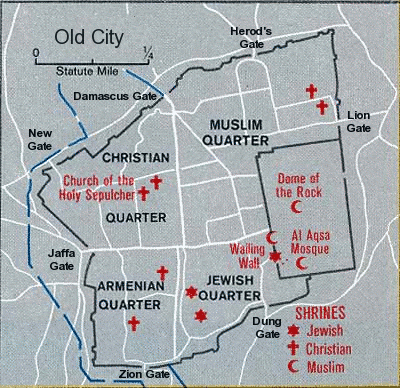
\includegraphics[width=0.5\textwidth]{MapJerusalemOldCity}

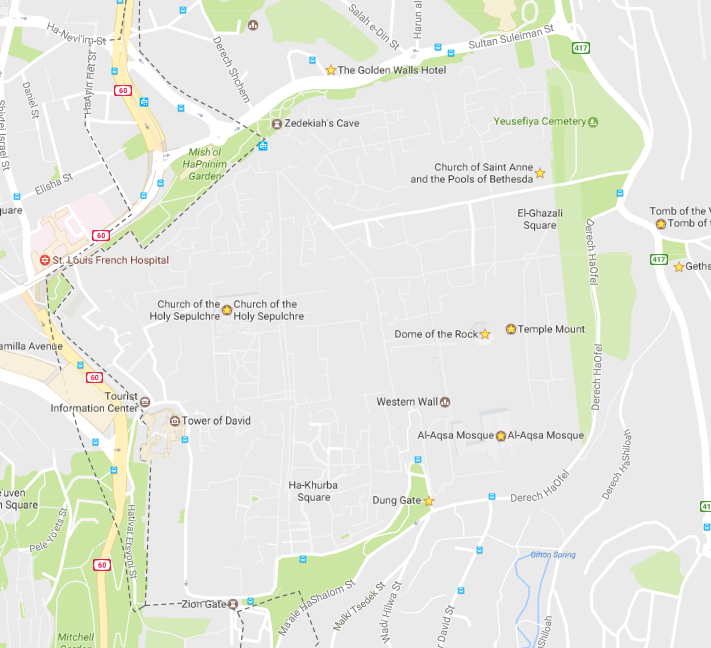
\includegraphics[width=\textwidth]{OldJerusalem}

\href{http://www.jesus-story.net/maps_jesus.htm}{
	This image shows the old city layout at the time of King Herod}

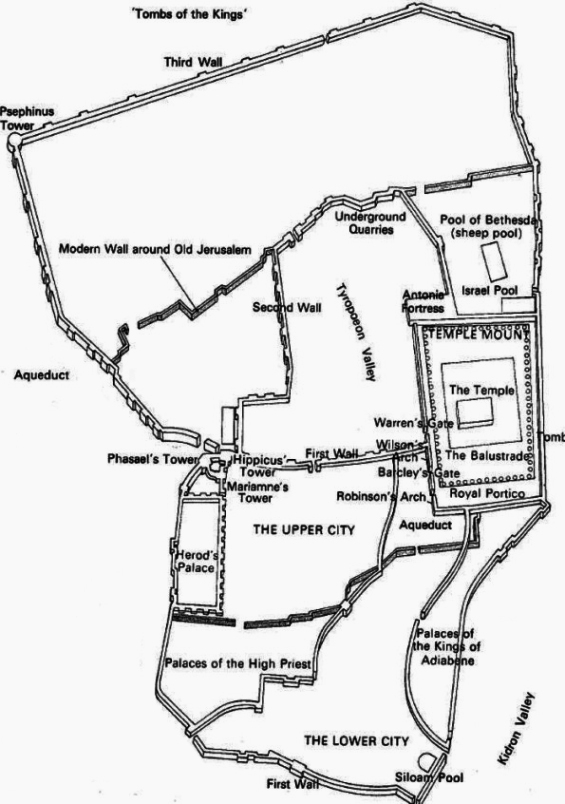
\includegraphics[height=0.9\textheight]{JerusalemAsItWas}

\clearpage
\subsection{The Upper Room}
\begin{multicols}{2}
	\mbox{}
\end{multicols}
\subsubsection{Scripture}

{\centering
	\emph{\bibleverse{Mark}(14:12-26) The Passover with the Disciples,
		The Institution of the Lord’s Supper,
		Peter’s Denial Foretold}\\
}
\begin{multicols}{2}
12 And on the first day of Unleavened Bread, when they sacrificed the passover lamb, his disciples said to him, “Where will you have us go and prepare for you to eat the passover?” 13 And he sent two of his disciples, and said to them, “Go into the city, and a man carrying a jar of water will meet you; follow him, 14 and wherever he enters, say to the householder, ‘The Teacher says, Where is my guest room, where I am to eat the passover with my disciples?’ 15 And he will show you a large upper room furnished and ready; there prepare for us.” 16 And the disciples set out and went to the city, and found it as he had told them; and they prepared the passover.

17 And when it was evening he came with the twelve. 18 And as they were at table eating, Jesus said, “Truly, I say to you, one of you will betray me, one who is eating with me.” 19 They began to be sorrowful, and to say to him one after another, “Is it I?” 20 He said to them, “It is one of the twelve, one who is dipping bread into the dish with me. 21 For the Son of man goes as it is written of him, but woe to that man by whom the Son of man is betrayed! It would have been better for that man if he had not been born.”

22 And as they were eating, he took bread, and blessed, and broke it, and gave it to them, and said, “Take; this is my body.” 23 And he took a cup, and when he had given thanks he gave it to them, and they all drank of it. 24 And he said to them, “This is my blood of the[a] covenant, which is poured out for many. 25 Truly, I say to you, I shall not drink again of the fruit of the vine until that day when I drink it new in the kingdom of God.”

26 And when they had sung a hymn, they went out to the Mount of Olives.
\end{multicols}

{\centering
	\emph{\bibleverse{Matthew}(26:17-30) The Passover with the Disciples,
		The Institution of the Lord’s Supper,
		Peter’s Denial Foretold}\\
}
\begin{multicols}{2}
17 Now on the first day of Unleavened Bread the disciples came to Jesus, saying, “Where will you have us prepare for you to eat the passover?” 18 He said, “Go into the city to a certain one, and say to him, ‘The Teacher says, My time is at hand; I will keep the passover at your house with my disciples.’” 19 And the disciples did as Jesus had directed them, and they prepared the passover.

20 When it was evening, he sat at table with the twelve disciples; 21 and as they were eating, he said, “Truly, I say to you, one of you will betray me.” 22 And they were very sorrowful, and began to say to him one after another, “Is it I, Lord?” 23 He answered, “He who has dipped his hand in the dish with me, will betray me. 24 The Son of man goes as it is written of him, but woe to that man by whom the Son of man is betrayed! It would have been better for that man if he had not been born.” 25 Judas, who betrayed him, said, “Is it I, Master?” He said to him, “You have said so.”

26 Now as they were eating, Jesus took bread, and blessed, and broke it, and gave it to the disciples and said, “Take, eat; this is my body.” 27 And he took a cup, and when he had given thanks he gave it to them, saying, “Drink of it, all of you; 28 for this is my blood of the covenant, which is poured out for many for the forgiveness of sins. 29 I tell you I shall not drink again of this fruit of the vine until that day when I drink it new with you in my Father’s kingdom.”

30 And when they had sung a hymn, they went out to the Mount of Olives.
\end{multicols}

{\centering
	\emph{\bibleverse{John}(13:1-17) Jesus Washes the Disciples’ Feet}\\
}
\begin{multicols}{2}
Now before the feast of the Passover, when Jesus knew that his hour had come to depart out of this world to the Father, having loved his own who were in the world, he loved them to the end. 2 And during supper, when the devil had already put it into the heart of Judas Iscariot, Simon’s son, to betray him, 3 Jesus, knowing that the Father had given all things into his hands, and that he had come from God and was going to God, 4 rose from supper, laid aside his garments, and girded himself with a towel. 5 Then he poured water into a basin, and began to wash the disciples’ feet, and to wipe them with the towel with which he was girded. 6 He came to Simon Peter; and Peter said to him, “Lord, do you wash my feet?” 7 Jesus answered him, “What I am doing you do not know now, but afterward you will understand.” 8 Peter said to him, “You shall never wash my feet.” Jesus answered him, “If I do not wash you, you have no part in me.” 9 Simon Peter said to him, “Lord, not my feet only but also my hands and my head!” 10 Jesus said to him, “He who has bathed does not need to wash, except for his feet,[a] but he is clean all over; and you[b] are clean, but not every one of you.” 11 For he knew who was to betray him; that was why he said, “You are not all clean.”

12 When he had washed their feet, and taken his garments, and resumed his place, he said to them, “Do you know what I have done to you? 13 You call me Teacher and Lord; and you are right, for so I am. 14 If I then, your Lord and Teacher, have washed your feet, you also ought to wash one another’s feet. 15 For I have given you an example, that you also should do as I have done to you. 16 Truly, truly, I say to you, a servant[c] is not greater than his master; nor is he who is sent greater than he who sent him. 17 If you know these things, blessed are you if you do them.
\end{multicols}

{\centering
	\emph{\bibleverse{Acts}(2:1-21) The Coming of the Holy Spirit,
		Peter Addresses the Crowd}\\
}
\begin{multicols}{2}
When the day of Pentecost had come, they were all together in one place. 2 And suddenly a sound came from heaven like the rush of a mighty wind, and it filled all the house where they were sitting. 3 And there appeared to them tongues as of fire, distributed and resting on each one of them. 4 And they were all filled with the Holy Spirit and began to speak in other tongues, as the Spirit gave them utterance.

5 Now there were dwelling in Jerusalem Jews, devout men from every nation under heaven. 6 And at this sound the multitude came together, and they were bewildered, because each one heard them speaking in his own language. 7 And they were amazed and wondered, saying, “Are not all these who are speaking Galileans? 8 And how is it that we hear, each of us in his own native language? 9 Par′thians and Medes and E′lamites and residents of Mesopota′mia, Judea and Cappado′cia, Pontus and Asia, 10 Phryg′ia and Pamphyl′ia, Egypt and the parts of Libya belonging to Cyre′ne, and visitors from Rome, both Jews and proselytes, 11 Cretans and Arabians, we hear them telling in our own tongues the mighty works of God.” 12 And all were amazed and perplexed, saying to one another, “What does this mean?” 13 But others mocking said, “They are filled with new wine.”

14 But Peter, standing with the eleven, lifted up his voice and addressed them, “Men of Judea and all who dwell in Jerusalem, let this be known to you, and give ear to my words. 15 For these men are not drunk, as you suppose, since it is only the third hour of the day; 16 but this is what was spoken by the prophet Joel:
\begin{verse}
17 ‘And in the last days it shall be, God declares,\\
that I will pour out my Spirit upon all flesh,\\
and your sons and your daughters shall prophesy,\\
and your young men shall see visions,\\
and your old men shall dream dreams;\\
18 yea, and on my menservants and my maidservants in those days\\
I will pour out my Spirit; and they shall prophesy.\\
19 And I will show wonders in the heaven above\\
and signs on the earth beneath,\\
blood, and fire, and vapor of smoke;\\
20 the sun shall be turned into darkness\\
and the moon into blood,\\
before the day of the Lord comes,\\
the great and manifest day.\\
21 And it shall be that whoever calls on the name of the Lord shall be saved.’\\
\end{verse}
\end{multicols}


\clearpage
\subsection{Pool of Bethesda}
\begin{multicols}{2}
	\mbox{}
\end{multicols}
\subsubsection{Scripture}

{\centering
	\emph{\bibleverse{John}(5:1-15) Jesus Heals on the Sabbath}\\
}
\begin{multicols}{2}
After this there was a feast of the Jews, and Jesus went up to Jerusalem.

2 Now there is in Jerusalem by the Sheep Gate a pool, in Hebrew called Beth-za′tha, which has five porticoes. 3 In these lay a multitude of invalids, blind, lame, paralyzed. 5 One man was there, who had been ill for thirty-eight years. 6 When Jesus saw him and knew that he had been lying there a long time, he said to him, “Do you want to be healed?” 7 The sick man answered him, “Sir, I have no man to put me into the pool when the water is troubled, and while I am going another steps down before me.” 8 Jesus said to him, “Rise, take up your pallet, and walk.” 9 And at once the man was healed, and he took up his pallet and walked.

Now that day was the sabbath. 10 So the Jews said to the man who was cured, “It is the sabbath, it is not lawful for you to carry your pallet.” 11 But he answered them, “The man who healed me said to me, ‘Take up your pallet, and walk.’” 12 They asked him, “Who is the man who said to you, ‘Take up your pallet, and walk’?” 13 Now the man who had been healed did not know who it was, for Jesus had withdrawn, as there was a crowd in the place. 14 Afterward, Jesus found him in the temple, and said to him, “See, you are well! Sin no more, that nothing worse befall you.” 15 The man went away and told the Jews that it was Jesus who had healed him.
\end{multicols}

\clearpage
\subsection{Pool of Siloam}
\begin{multicols}{2}
	\mbox{}
\end{multicols}
\subsubsection{Scripture}

{\centering
	\emph{\bibleverse{John}(9:1-38) A Man Born Blind Receives Sight,
		The Pharisees Investigate the Healing, Spiritual Blindness}\\
}
\begin{multicols}{2}
As he passed by, he saw a man blind from his birth. 2 And his disciples asked him, “Rabbi, who sinned, this man or his parents, that he was born blind?” 3 Jesus answered, “It was not that this man sinned, or his parents, but that the works of God might be made manifest in him. 4 We must work the works of him who sent me, while it is day; night comes, when no one can work. 5 As long as I am in the world, I am the light of the world.” 6 As he said this, he spat on the ground and made clay of the spittle and anointed the man’s eyes with the clay, 7 saying to him, “Go, wash in the pool of Silo′am” (which means Sent). So he went and washed and came back seeing. 8 The neighbors and those who had seen him before as a beggar, said, “Is not this the man who used to sit and beg?” 9 Some said, “It is he”; others said, “No, but he is like him.” He said, “I am the man.” 10 They said to him, “Then how were your eyes opened?” 11 He answered, “The man called Jesus made clay and anointed my eyes and said to me, ‘Go to Silo′am and wash’; so I went and washed and received my sight.” 12 They said to him, “Where is he?” He said, “I do not know.”

13 They brought to the Pharisees the man who had formerly been blind. 14 Now it was a sabbath day when Jesus made the clay and opened his eyes. 15 The Pharisees again asked him how he had received his sight. And he said to them, “He put clay on my eyes, and I washed, and I see.” 16 Some of the Pharisees said, “This man is not from God, for he does not keep the sabbath.” But others said, “How can a man who is a sinner do such signs?” There was a division among them. 17 So they again said to the blind man, “What do you say about him, since he has opened your eyes?” He said, “He is a prophet.”

18 The Jews did not believe that he had been blind and had received his sight, until they called the parents of the man who had received his sight, 19 and asked them, “Is this your son, who you say was born blind? How then does he now see?” 20 His parents answered, “We know that this is our son, and that he was born blind; 21 but how he now sees we do not know, nor do we know who opened his eyes. Ask him; he is of age, he will speak for himself.” 22 His parents said this because they feared the Jews, for the Jews had already agreed that if any one should confess him to be Christ, he was to be put out of the synagogue. 23 Therefore his parents said, “He is of age, ask him.”

24 So for the second time they called the man who had been blind, and said to him, “Give God the praise; we know that this man is a sinner.” 25 He answered, “Whether he is a sinner, I do not know; one thing I know, that though I was blind, now I see.” 26 They said to him, “What did he do to you? How did he open your eyes?” 27 He answered them, “I have told you already, and you would not listen. Why do you want to hear it again? Do you too want to become his disciples?” 28 And they reviled him, saying, “You are his disciple, but we are disciples of Moses. 29 We know that God has spoken to Moses, but as for this man, we do not know where he comes from.” 30 The man answered, “Why, this is a marvel! You do not know where he comes from, and yet he opened my eyes. 31 We know that God does not listen to sinners, but if any one is a worshiper of God and does his will, God listens to him. 32 Never since the world began has it been heard that any one opened the eyes of a man born blind. 33 If this man were not from God, he could do nothing.” 34 They answered him, “You were born in utter sin, and would you teach us?” And they cast him out.

35 Jesus heard that they had cast him out, and having found him he said, “Do you believe in the Son of man?”[a] 36 He answered, “And who is he, sir, that I may believe in him?” 37 Jesus said to him, “You have seen him, and it is he who speaks to you.” 38 He said, “Lord, I believe”; and he worshiped him.
\end{multicols}

\clearpage
\subsection{Church of the Holy Sepulchre}
\begin{multicols}{2}
	\mbox{}
\end{multicols}
\subsubsection{Scripture}
{\centering
	The Anointing Stone inside the entrance
	
	\emph{\bibleverse{Mark}(15:42-47) The Burial of Jesus}\\
}
\begin{multicols}{2}
	42 And when evening had come, since it was the day of Preparation, that is, the day before the sabbath, 43 Joseph of Arimathe′a, a respected member of the council, who was also himself looking for the kingdom of God, took courage and went to Pilate, and asked for the body of Jesus. 44 And Pilate wondered if he were already dead; and summoning the centurion, he asked him whether he was already dead.[a] 45 And when he learned from the centurion that he was dead, he granted the body to Joseph. 46 And he bought a linen shroud, and taking him down, wrapped him in the linen shroud, and laid him in a tomb which had been hewn out of the rock; and he rolled a stone against the door of the tomb. 47 Mary Mag′dalene and Mary the mother of Joses saw where he was laid.
\end{multicols}

{\centering
	Golgotha...each evangelist has a passage announcing this
	
	\emph{\bibleverse{Matthew}(27:27-56) The Soldiers Mock Jesus, The Crucifixion of Jesus, The Death of Jesus}\\
}
\begin{multicols}{2}
27 Then the soldiers of the governor took Jesus into the praetorium, and they gathered the whole battalion before him. 28 And they stripped him and put a scarlet robe upon him, 29 and plaiting a crown of thorns they put it on his head, and put a reed in his right hand. And kneeling before him they mocked him, saying, “Hail, King of the Jews!” 30 And they spat upon him, and took the reed and struck him on the head. 31 And when they had mocked him, they stripped him of the robe, and put his own clothes on him, and led him away to crucify him.

32 As they went out, they came upon a man of Cyre′ne, Simon by name; this man they compelled to carry his cross. 33 And when they came to a place called Gol′gotha (which means the place of a skull), 34 they offered him wine to drink, mingled with gall; but when he tasted it, he would not drink it. 35 And when they had crucified him, they divided his garments among them by casting lots; 36 then they sat down and kept watch over him there. 37 And over his head they put the charge against him, which read, “This is Jesus the King of the Jews.” 38 Then two robbers were crucified with him, one on the right and one on the left. 39 And those who passed by derided him, wagging their heads 40 and saying, “You who would destroy the temple and build it in three days, save yourself! If you are the Son of God, come down from the cross.” 41 So also the chief priests, with the scribes and elders, mocked him, saying, 42 “He saved others; he cannot save himself. He is the King of Israel; let him come down now from the cross, and we will believe in him. 43 He trusts in God; let God deliver him now, if he desires him; for he said, ‘I am the Son of God.’” 44 And the robbers who were crucified with him also reviled him in the same way.

45 Now from the sixth hour there was darkness over all the land until the ninth hour. 46 And about the ninth hour Jesus cried with a loud voice, “Eli, Eli, la′ma sabach-tha′ni?” that is, “My God, my God, why hast thou forsaken me?” 47 And some of the bystanders hearing it said, “This man is calling Eli′jah.” 48 And one of them at once ran and took a sponge, filled it with vinegar, and put it on a reed, and gave it to him to drink. 49 But the others said, “Wait, let us see whether Eli′jah will come to save him.” 50 And Jesus cried again with a loud voice and yielded up his spirit.

51 And behold, the curtain of the temple was torn in two, from top to bottom; and the earth shook, and the rocks were split; 52 the tombs also were opened, and many bodies of the saints who had fallen asleep were raised, 53 and coming out of the tombs after his resurrection they went into the holy city and appeared to many. 54 When the centurion and those who were with him, keeping watch over Jesus, saw the earthquake and what took place, they were filled with awe, and said, “Truly this was the Son of God!”

55 There were also many women there, looking on from afar, who had followed Jesus from Galilee, ministering to him; 56 among whom were Mary Mag′dalene, and Mary the mother of James and Joseph, and the mother of the sons of Zeb′edee.
\end{multicols}

{\centering
	The Life-Giving Tomb of Christ
	
	\emph{\bibleverse{Mark}(15:42-16:8) The Burial of Jesus,
		The Resurrection of Jesus,}\\
}
\begin{multicols}{2}
42 And when evening had come, since it was the day of Preparation, that is, the day before the sabbath, 43 Joseph of Arimathe′a, a respected member of the council, who was also himself looking for the kingdom of God, took courage and went to Pilate, and asked for the body of Jesus. 44 And Pilate wondered if he were already dead; and summoning the centurion, he asked him whether he was already dead. 45 And when he learned from the centurion that he was dead, he granted the body to Joseph. 46 And he bought a linen shroud, and taking him down, wrapped him in the linen shroud, and laid him in a tomb which had been hewn out of the rock; and he rolled a stone against the door of the tomb. 47 Mary Mag′dalene and Mary the mother of Joses saw where he was laid.

16 And when the sabbath was past, Mary Mag′dalene, and Mary the mother of James, and Salo′me, bought spices, so that they might go and anoint him. 2 And very early on the first day of the week they went to the tomb when the sun had risen. 3 And they were saying to one another, “Who will roll away the stone for us from the door of the tomb?” 4 And looking up, they saw that the stone was rolled back—it was very large. 5 And entering the tomb, they saw a young man sitting on the right side, dressed in a white robe; and they were amazed. 6 And he said to them, “Do not be amazed; you seek Jesus of Nazareth, who was crucified. He has risen, he is not here; see the place where they laid him. 7 But go, tell his disciples and Peter that he is going before you to Galilee; there you will see him, as he told you.” 8 And they went out and fled from the tomb; for trembling and astonishment had come upon them; and they said nothing to any one, for they were afraid.
\end{multicols}

\clearpage
\subsection{Daily Notes}

\clearpage
\subsection{Journal Entry}

%%%%%%%%%%%%%%%%%%%%%%%%%%%%%%%%%%%%%%%%%%%%%%%%%%%%%%%%%%%%%%%%%%%%%%%%%%%%%%%
\clearpage
\section{Jan 28 - Saturday - Day 4}
To the East of Jerusalem: Jordan, Jericho, \& Dead Sea

\subsection{Agenda}
\begin{description}
	\item[08:00am]  Monastery of St. Gerasimos
	  \subitem Qasr el-Yahud baptismal site on the River Jordan
	    (renewal of baptismal vows)
	  \subitem Service at the baptismal site in Qasr el-Yahud
	  \subitem Opportunity to swim (float) in the Dead Sea
	\item[Lunch] in Jericho at the Al-Rawda Restaurant 
	\item[Afternoon] Desert oasis of Jericho: Tree of Zacchaeus – Monastery of the Prophet Elijah
	  \subitem Cable car up Mount of Temptation
	  \subitem Monastery of Sarantario (Temptation)
	  \subitem Wadi Qelt: view St. George's Monastery (walk down if situation \& time permits) 
	\item[Hotel] Dinner \& overnight in Jerusalem at the
	  \href{http://goldenwalls.com/}{Golden Walls Hotel}
	\item[23:00]  Church of the Holy Sepulchre – Midnight Liturgy
\end{description}

\subsection{Notes from Fr. Gregory}
After breakfast, we depart for the Monastery of St. Gerasimos...
here is a nice little feature to give everyone some background about this
saint and this site:

\url{http://www.biblewalks.com/Sites/StGerassimos.html}
or

\url{http://www.seetheholyland.net/monastery-of-st-gerasimus/}

(This monastery is built over the site believed to house a cave where the Holy 
Family stayed as they fled to Egypt and is also famous for being the monastery 
of St. Zosimas, who traveled into the desert and met St. Mary of Egypt).

We then travel to Qasr el-Yahud where we will visit the Jordan River and 
celebrate the Outdoor Blessing of Water...
some people enjoy actually entering the river completely and being blessed
with these holy waters.
(Matthew 3:13-17; Mark 1:9-11; Luke 3:21-23.

Anyone who might wish to experience "swimming" in the Dead Sea
(more like floating) should be prepared to do it on this day...
in other words, swim atire would be good today.

After lunch in Jericho,
we will visit the Tree of Zacchaeus and Monastery of the Prophet Elijah,
Luke 19:1-10;
Monastery of the Mount of Temptation (Luke 4:1-14)
and Monastery of St. George in Wadi Qelt (Elijah's Cave)
(we will walk down if time permits)...
\url{https://en.wikipedia.org/wiki/St._George's_Monastery,_Wadi_Qelt}

We return to the hotel for dinner and a little rest before departing for 
Liturgy at the Holy Sepulchre (optional)
to be there by 11pm for the Liturgy at Midnight...time may vary.

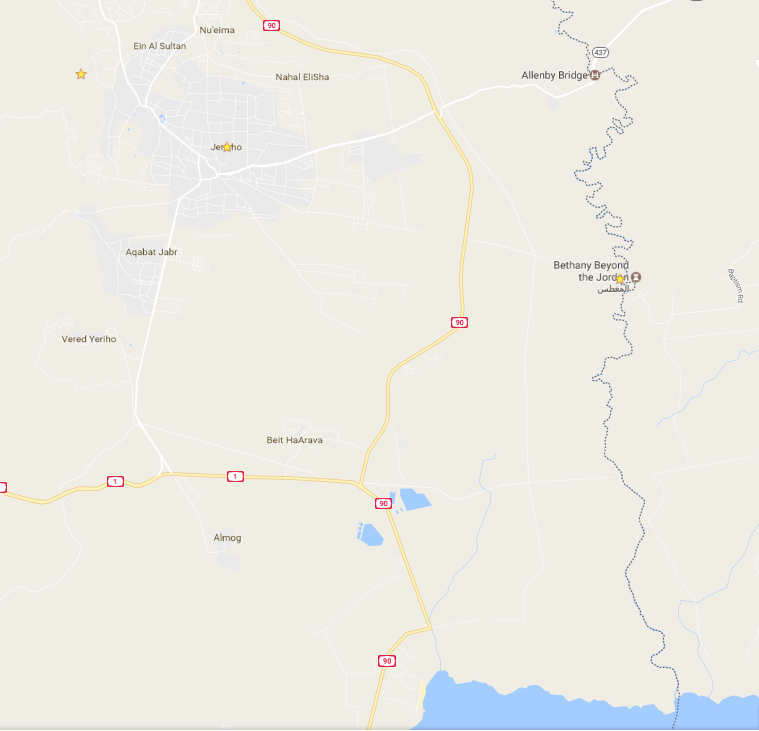
\includegraphics[width=\textwidth]{JordanDeadseaJerichoTemptation}

\clearpage
\subsection{Jordan River -- Qasr el-Yahud}
\begin{multicols}{2}
	\mbox{}
\end{multicols}
\subsubsection{Scripture}

{\centering
	\emph{\bibleverse{Matthew}(3:13-17) The Baptism of Jesus}\\
}
\begin{multicols}{2}
13 Then Jesus came from Galilee to the Jordan to John, to be baptized by him. 14 John would have prevented him, saying, “I need to be baptized by you, and do you come to me?” 15 But Jesus answered him, “Let it be so now; for thus it is fitting for us to fulfil all righteousness.” Then he consented. 16 And when Jesus was baptized, he went up immediately from the water, and behold, the heavens were opened and he saw the Spirit of God descending like a dove, and alighting on him; 17 and lo, a voice from heaven, saying, “This is my beloved Son, with whom I am well pleased.”
\end{multicols}

{\centering
	\emph{\bibleverse{Mark}(1:9-11) The Baptism of Jesus}\\
}
\begin{multicols}{2}
9 In those days Jesus came from Nazareth of Galilee and was baptized by John in the Jordan. 10 And when he came up out of the water, immediately he saw the heavens opened and the Spirit descending upon him like a dove; 11 and a voice came from heaven, “Thou art my beloved Son; with thee I am well pleased.”
\end{multicols}

{\centering
	\emph{\bibleverse{Luke}(3:21-23) The Baptism of Jesus}\\
}
\begin{multicols}{2}
21 Now when all the people were baptized, and when Jesus also had been baptized and was praying, the heaven was opened, 22 and the Holy Spirit descended upon him in bodily form, as a dove, and a voice came from heaven, “Thou art my beloved Son;[a] with thee I am well pleased.”

23 Jesus, when he began his ministry, was about thirty years of age, being the son (as was supposed) of Joseph, the son of Heli,
\end{multicols}

\clearpage
\subsection{Tree of Zacchaeus and Monastery of the Prophet Elijah}
\begin{multicols}{2}
	\mbox{}
\end{multicols}
\subsubsection{Scripture}

{\centering
	\emph{\bibleverse{Luke}(19:1-10) Jesus and Zacchaeus}\\
}
\begin{multicols}{2}
19 He entered Jericho and was passing through. 2 And there was a man named Zacchae′us; he was a chief tax collector, and rich. 3 And he sought to see who Jesus was, but could not, on account of the crowd, because he was small of stature. 4 So he ran on ahead and climbed up into a sycamore tree to see him, for he was to pass that way. 5 And when Jesus came to the place, he looked up and said to him, “Zacchae′us, make haste and come down; for I must stay at your house today.” 6 So he made haste and came down, and received him joyfully. 7 And when they saw it they all murmured, “He has gone in to be the guest of a man who is a sinner.” 8 And Zacchae′us stood and said to the Lord, “Behold, Lord, the half of my goods I give to the poor; and if I have defrauded any one of anything, I restore it fourfold.” 9 And Jesus said to him, “Today salvation has come to this house, since he also is a son of Abraham. 10 For the Son of man came to seek and to save the lost.”
\end{multicols}

\clearpage
\subsection{Monastery of Sarantario (Temptation)}
\begin{multicols}{2}
	\mbox{}
\end{multicols}
\subsubsection{Scripture}

{\centering
	\emph{\bibleverse{Luke}(4:1-14) The Temptation of Jesus,
		The Beginning of the Galilean Ministry}\\
}
\begin{multicols}{2}
And Jesus, full of the Holy Spirit, returned from the Jordan, and was led by the Spirit 2 for forty days in the wilderness, tempted by the devil. And he ate nothing in those days; and when they were ended, he was hungry. 3 The devil said to him, “If you are the Son of God, command this stone to become bread.” 4 And Jesus answered him, “It is written, ‘Man shall not live by bread alone.’” 5 And the devil took him up, and showed him all the kingdoms of the world in a moment of time, 6 and said to him, “To you I will give all this authority and their glory; for it has been delivered to me, and I give it to whom I will. 7 If you, then, will worship me, it shall all be yours.” 8 And Jesus answered him, “It is written,

\begin{verse}
‘You shall worship the Lord your God,\\
and him only shall you serve.’”\\
\end{verse}

9 And he took him to Jerusalem, and set him on the pinnacle of the temple, and said to him, “If you are the Son of God, throw yourself down from here; 10 for it is written,

\begin{verse}
‘He will give his angels charge of you, to guard you,’\\
\end{verse}

11 and

\begin{verse}
‘On their hands they will bear you up,\\
lest you strike your foot against a stone.’”\\
\end{verse}

12 And Jesus answered him, “It is said, ‘You shall not tempt the Lord your God.’” 13 And when the devil had ended every temptation, he departed from him until an opportune time.

14 And Jesus returned in the power of the Spirit into Galilee, and a report concerning him went out through all the surrounding country.

\end{multicols}

\clearpage
\subsection{Daily Notes}

\clearpage
\subsection{Journal Entry}

%%%%%%%%%%%%%%%%%%%%%%%%%%%%%%%%%%%%%%%%%%%%%%%%%%%%%%%%%%%%%%%%%%%%%%%%%%%%%%%
\clearpage
\section{Jan 29 - Sunday - Day 5}
More North -- To the Sea of Galilee
\subsection{Agenda}
\begin{description}
	\item[08:00am] Check-out of the hotel Bethany
	  \subitem Church \& tomb of Lazarus – Monastery of Martha \& Mary
	  \subitem Drive to Galilee via the West Bank and Nablus
	\item[Lunch] in Sebastia at the Samaria Restaurant
	\item[Afternoon] Ruins of Sebastia – Nablus: Jacob’s Well
	  \subitem Continue to the Sea of Galile
	\item[Hotel] Dinner \& overnight in Tiberias at the
	  \href{http://www.ronbeachhotel.com/}{Ron Beach Hotel}.
\end{description}

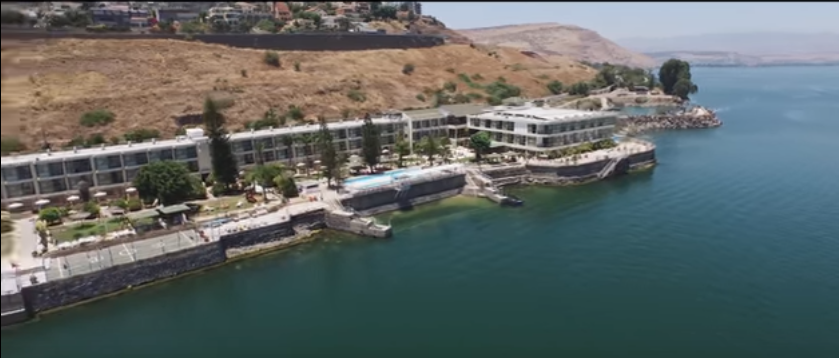
\includegraphics[width=\textwidth]{RonBeachHotel}

\subsection{Notes from Fr. Gregory}
We check out of the hotel in Jerusalem and head for Bethany to visit the 
Church and Tomb of Lazarus and the Monastery of Martha and Mary.
John 11:1-45

After Lunch in Samaria, we visit Sebastia (Nablus)...Jacob's
Well and Prison of St John the Baptist (John 4:5-42 and Mark 6:14-29). Go to
\url{https://en.wikipedia.org/wiki/Jacob's_Well}.

We will then continue to the city of Tiberias on the Sea of Galilee for dinner 
and overnight at the Ron Beach Hotel.

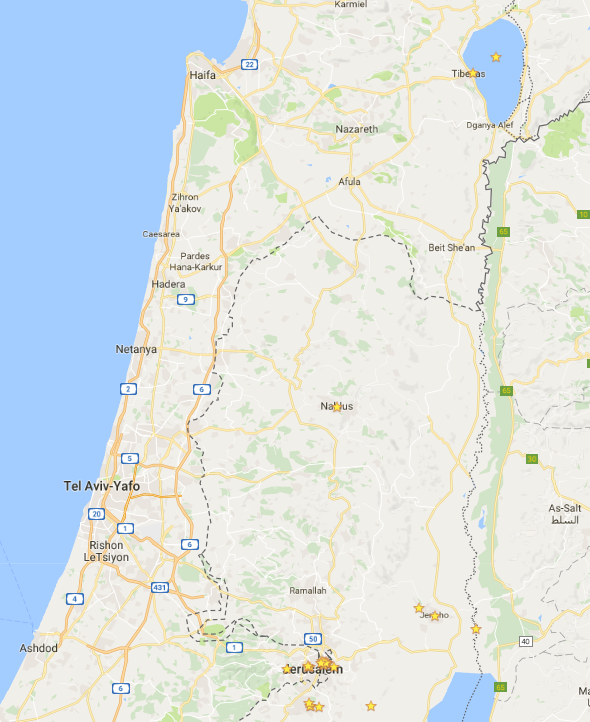
\includegraphics[height=\textheight]{JerusalemSeaOfGalile}


\clearpage
\subsection{Tomb of Lazarus -- Monastery of Martha \& Mary}
\begin{multicols}{2}
	\mbox{}
\end{multicols}
\subsubsection{Scripture}

{\centering
	\emph{\bibleverse{John}(11:1-45) The Death of Lazarus,
		Jesus the Resurrection and the Life,
		Jesus Weeps,
		Jesus Raises Lazarus to Life,
		The Plot to Kill Jesus}\\
}
\begin{multicols}{2}
Now a certain man was ill, Laz′arus of Bethany, the village of Mary and her sister Martha. 2 It was Mary who anointed the Lord with ointment and wiped his feet with her hair, whose brother Laz′arus was ill. 3 So the sisters sent to him, saying, “Lord, he whom you love is ill.” 4 But when Jesus heard it he said, “This illness is not unto death; it is for the glory of God, so that the Son of God may be glorified by means of it.”

5 Now Jesus loved Martha and her sister and Laz′arus. 6 So when he heard that he was ill, he stayed two days longer in the place where he was. 7 Then after this he said to the disciples, “Let us go into Judea again.” 8 The disciples said to him, “Rabbi, the Jews were but now seeking to stone you, and are you going there again?” 9 Jesus answered, “Are there not twelve hours in the day? If any one walks in the day, he does not stumble, because he sees the light of this world. 10 But if any one walks in the night, he stumbles, because the light is not in him.” 11 Thus he spoke, and then he said to them, “Our friend Laz′arus has fallen asleep, but I go to awake him out of sleep.” 12 The disciples said to him, “Lord, if he has fallen asleep, he will recover.” 13 Now Jesus had spoken of his death, but they thought that he meant taking rest in sleep. 14 Then Jesus told them plainly, “Laz′arus is dead; 15 and for your sake I am glad that I was not there, so that you may believe. But let us go to him.” 16 Thomas, called the Twin, said to his fellow disciples, “Let us also go, that we may die with him.”

17 Now when Jesus came, he found that Laz′arus[a] had already been in the tomb four days. 18 Bethany was near Jerusalem, about two miles[b] off, 19 and many of the Jews had come to Martha and Mary to console them concerning their brother. 20 When Martha heard that Jesus was coming, she went and met him, while Mary sat in the house. 21 Martha said to Jesus, “Lord, if you had been here, my brother would not have died. 22 And even now I know that whatever you ask from God, God will give you.” 23 Jesus said to her, “Your brother will rise again.” 24 Martha said to him, “I know that he will rise again in the resurrection at the last day.” 25 Jesus said to her, “I am the resurrection and the life;[c] he who believes in me, though he die, yet shall he live, 26 and whoever lives and believes in me shall never die. Do you believe this?” 27 She said to him, “Yes, Lord; I believe that you are the Christ, the Son of God, he who is coming into the world.”

28 When she had said this, she went and called her sister Mary, saying quietly, “The Teacher is here and is calling for you.” 29 And when she heard it, she rose quickly and went to him. 30 Now Jesus had not yet come to the village, but was still in the place where Martha had met him. 31 When the Jews who were with her in the house, consoling her, saw Mary rise quickly and go out, they followed her, supposing that she was going to the tomb to weep there. 32 Then Mary, when she came where Jesus was and saw him, fell at his feet, saying to him, “Lord, if you had been here, my brother would not have died.” 33 When Jesus saw her weeping, and the Jews who came with her also weeping, he was deeply moved in spirit and troubled; 34 and he said, “Where have you laid him?” They said to him, “Lord, come and see.” 35 Jesus wept. 36 So the Jews said, “See how he loved him!” 37 But some of them said, “Could not he who opened the eyes of the blind man have kept this man from dying?”

38 Then Jesus, deeply moved again, came to the tomb; it was a cave, and a stone lay upon it. 39 Jesus said, “Take away the stone.” Martha, the sister of the dead man, said to him, “Lord, by this time there will be an odor, for he has been dead four days.” 40 Jesus said to her, “Did I not tell you that if you would believe you would see the glory of God?” 41 So they took away the stone. And Jesus lifted up his eyes and said, “Father, I thank thee that thou hast heard me. 42 I knew that thou hearest me always, but I have said this on account of the people standing by, that they may believe that thou didst send me.” 43 When he had said this, he cried with a loud voice, “Laz′arus, come out.” 44 The dead man came out, his hands and feet bound with bandages, and his face wrapped with a cloth. Jesus said to them, “Unbind him, and let him go.”

45 Many of the Jews therefore, who had come with Mary and had seen what he did, believed in him;
\end{multicols}

\clearpage
\subsection{Jacob's Well}
\begin{multicols}{2}
	\mbox{}
\end{multicols}
\subsubsection{Scripture}

{\centering
	\emph{\bibleverse{John}(4:1-42) Jesus and the Woman of Samaria}\\
}
\begin{multicols}{2}
Now when the Lord knew that the Pharisees had heard that Jesus was making and baptizing more disciples than John 2 (although Jesus himself did not baptize, but only his disciples), 3 he left Judea and departed again to Galilee. 4 He had to pass through Samar′ia. 5 So he came to a city of Samar′ia, called Sy′char, near the field that Jacob gave to his son Joseph. 6 Jacob’s well was there, and so Jesus, wearied as he was with his journey, sat down beside the well. It was about the sixth hour.

7 There came a woman of Samar′ia to draw water. Jesus said to her, “Give me a drink.” 8 For his disciples had gone away into the city to buy food. 9 The Samaritan woman said to him, “How is it that you, a Jew, ask a drink of me, a woman of Samar′ia?” For Jews have no dealings with Samaritans. 10 Jesus answered her, “If you knew the gift of God, and who it is that is saying to you, ‘Give me a drink,’ you would have asked him, and he would have given you living water.” 11 The woman said to him, “Sir, you have nothing to draw with, and the well is deep; where do you get that living water? 12 Are you greater than our father Jacob, who gave us the well, and drank from it himself, and his sons, and his cattle?” 13 Jesus said to her, “Every one who drinks of this water will thirst again, 14 but whoever drinks of the water that I shall give him will never thirst; the water that I shall give him will become in him a spring of water welling up to eternal life.” 15 The woman said to him, “Sir, give me this water, that I may not thirst, nor come here to draw.”

16 Jesus said to her, “Go, call your husband, and come here.” 17 The woman answered him, “I have no husband.” Jesus said to her, “You are right in saying, ‘I have no husband’; 18 for you have had five husbands, and he whom you now have is not your husband; this you said truly.” 19 The woman said to him, “Sir, I perceive that you are a prophet. 20 Our fathers worshiped on this mountain; and you say that in Jerusalem is the place where men ought to worship.” 21 Jesus said to her, “Woman, believe me, the hour is coming when neither on this mountain nor in Jerusalem will you worship the Father. 22 You worship what you do not know; we worship what we know, for salvation is from the Jews. 23 But the hour is coming, and now is, when the true worshipers will worship the Father in spirit and truth, for such the Father seeks to worship him. 24 God is spirit, and those who worship him must worship in spirit and truth.” 25 The woman said to him, “I know that Messiah is coming (he who is called Christ); when he comes, he will show us all things.” 26 Jesus said to her, “I who speak to you am he.”

27 Just then his disciples came. They marveled that he was talking with a woman, but none said, “What do you wish?” or, “Why are you talking with her?” 28 So the woman left her water jar, and went away into the city, and said to the people, 29 “Come, see a man who told me all that I ever did. Can this be the Christ?” 30 They went out of the city and were coming to him.

31 Meanwhile the disciples besought him, saying, “Rabbi, eat.” 32 But he said to them, “I have food to eat of which you do not know.” 33 So the disciples said to one another, “Has any one brought him food?” 34 Jesus said to them, “My food is to do the will of him who sent me, and to accomplish his work. 35 Do you not say, ‘There are yet four months, then comes the harvest’? I tell you, lift up your eyes, and see how the fields are already white for harvest. 36 He who reaps receives wages, and gathers fruit for eternal life, so that sower and reaper may rejoice together. 37 For here the saying holds true, ‘One sows and another reaps.’ 38 I sent you to reap that for which you did not labor; others have labored, and you have entered into their labor.”

39 Many Samaritans from that city believed in him because of the woman’s testimony, “He told me all that I ever did.” 40 So when the Samaritans came to him, they asked him to stay with them; and he stayed there two days. 41 And many more believed because of his word. 42 They said to the woman, “It is no longer because of your words that we believe, for we have heard for ourselves, and we know that this is indeed the Savior of the world.”
\end{multicols}

\clearpage
\subsection{Prison of St John the Baptist}
\begin{multicols}{2}
	\mbox{}
\end{multicols}
\subsubsection{Scripture}

{\centering
	\emph{\bibleverse{Mark}(6:14-29) The Death of John the Baptist}\\
}
\begin{multicols}{2}
14 King Herod heard of it; for Jesus’[a] name had become known. Some[b] said, “John the baptizer has been raised from the dead; that is why these powers are at work in him.” 15 But others said, “It is Eli′jah.” And others said, “It is a prophet, like one of the prophets of old.” 16 But when Herod heard of it he said, “John, whom I beheaded, has been raised.” 17 For Herod had sent and seized John, and bound him in prison for the sake of Hero′di-as, his brother Philip’s wife; because he had married her. 18 For John said to Herod, “It is not lawful for you to have your brother’s wife.” 19 And Hero′di-as had a grudge against him, and wanted to kill him. But she could not, 20 for Herod feared John, knowing that he was a righteous and holy man, and kept him safe. When he heard him, he was much perplexed; and yet he heard him gladly. 21 But an opportunity came when Herod on his birthday gave a banquet for his courtiers and officers and the leading men of Galilee. 22 For when Hero′di-as’ daughter came in and danced, she pleased Herod and his guests; and the king said to the girl, “Ask me for whatever you wish, and I will grant it.” 23 And he vowed to her, “Whatever you ask me, I will give you, even half of my kingdom.” 24 And she went out, and said to her mother, “What shall I ask?” And she said, “The head of John the baptizer.” 25 And she came in immediately with haste to the king, and asked, saying, “I want you to give me at once the head of John the Baptist on a platter.” 26 And the king was exceedingly sorry; but because of his oaths and his guests he did not want to break his word to her. 27 And immediately the king sent a soldier of the guard and gave orders to bring his head. He went and beheaded him in the prison, 28 and brought his head on a platter, and gave it to the girl; and the girl gave it to her mother. 29 When his disciples heard of it, they came and took his body, and laid it in a tomb.
\end{multicols}

\clearpage
\subsection{Daily Notes}

\clearpage
\subsection{Journal Entry}

%%%%%%%%%%%%%%%%%%%%%%%%%%%%%%%%%%%%%%%%%%%%%%%%%%%%%%%%%%%%%%%%%%%%%%%%%%%%%%%
\clearpage
\section{Jan 30 - Monday - Day 6}
Around the Sea of Galilee - Capernaum

\subsection{Agenda}
\begin{description}
	\item[08:00am]  Greek Orthodox Church of Sts. Peter and Paul in Tiberias 
	  \subitem Greek Orthodox Church of the Apostles in Capernaum
	  \subitem Site of the healing of the paralytic
	  \subitem Beitsaida – Kursi
	      (associated with the story of the Gadarene swine…optional)
	  \subitem Ruins of Capernaum (Catholic site – optional) 
	\item[Lunch] Lunch by the lake at the St. Peter Restaurant
	\item[Afternoon] Church of the Loaves and Fishes at Tabgha Mount of 
	     Beatitudes
	\item[16:00] Sail on the Sea of Galilee to the Ron Beach Hotel
	\item[Hotel] Dinner \& overnight in Tiberias at the
	  \href{http://www.ronbeachhotel.com/}{Ron Beach Hotel}.
\end{description}

\subsection{Notes from Fr. Gregory}
After breakfast, we will visit the Greek Orthodox Churches of
Sts. Peter and Paul in Tiberias and the Church of the Apostles in Capernaum
(site of the healing of the paralytic).
Read Mark 2:1-12.

We may also visit other sites in Capernaum (Mark 1:21-31).
After lunch, we will visit Tabgha and the Church of the Loaves and Fishes
(Matthew 14:14-21 or John 6:5-14).

We also visit the Mount of the Beatitudes (Matthew 5:1-12).

We finish the day with a boat ride across the Sea of Galilee back to our hotel 
in Tiberias.

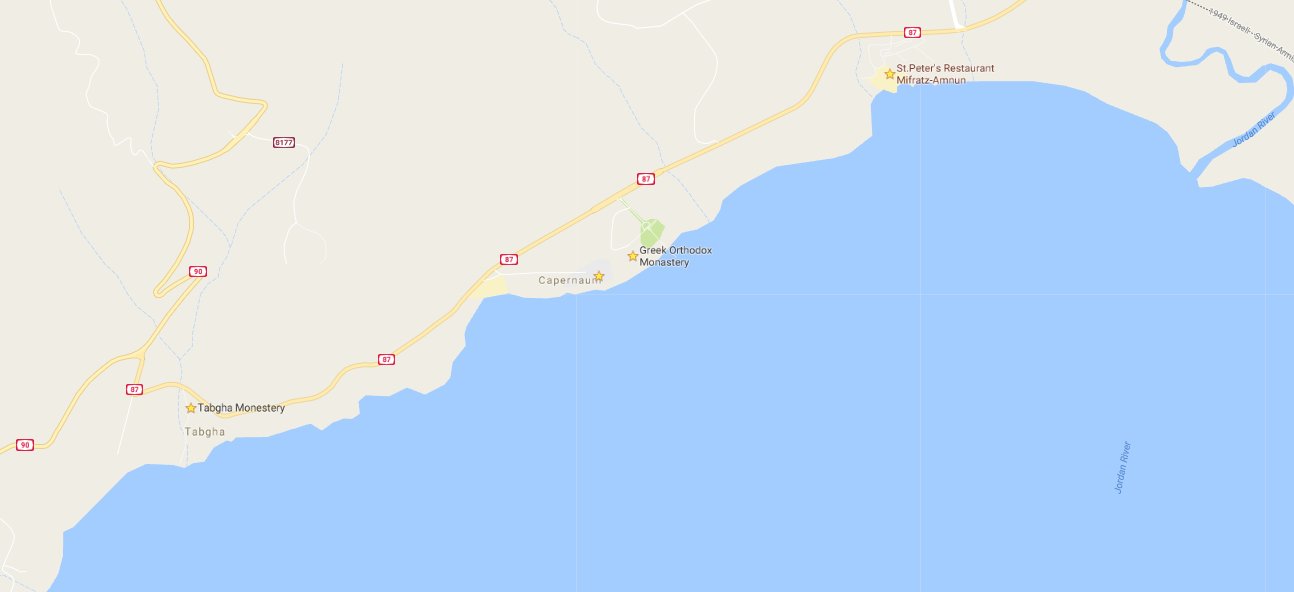
\includegraphics[width=\textwidth]{Capernaum}


\clearpage
\subsection{Church of the Apostles in Capernaum}
\begin{multicols}{2}
	\mbox{}
\end{multicols}
\subsubsection{Scripture}

{\centering
	\emph{\bibleverse{Mark}(2:1-12) Jesus Heals a Paralytic}\\
}
\begin{multicols}{2}
And when he returned to Caper′na-um after some days, it was reported that he was at home. 2 And many were gathered together, so that there was no longer room for them, not even about the door; and he was preaching the word to them. 3 And they came, bringing to him a paralytic carried by four men. 4 And when they could not get near him because of the crowd, they removed the roof above him; and when they had made an opening, they let down the pallet on which the paralytic lay. 5 And when Jesus saw their faith, he said to the paralytic, “My son, your sins are forgiven.” 6 Now some of the scribes were sitting there, questioning in their hearts, 7 “Why does this man speak thus? It is blasphemy! Who can forgive sins but God alone?” 8 And immediately Jesus, perceiving in his spirit that they thus questioned within themselves, said to them, “Why do you question thus in your hearts? 9 Which is easier, to say to the paralytic, ‘Your sins are forgiven,’ or to say, ‘Rise, take up your pallet and walk’? 10 But that you may know that the Son of man has authority on earth to forgive sins”—he said to the paralytic— 11 “I say to you, rise, take up your pallet and go home.” 12 And he rose, and immediately took up the pallet and went out before them all; so that they were all amazed and glorified God, saying, “We never saw anything like this!”
\end{multicols}

\clearpage
\subsection{Ruins of Capernaum (Catholic site – optional)}
\begin{multicols}{2}
	\mbox{}
\end{multicols}
\subsubsection{Scripture}

{\centering
	\emph{\bibleverse{Mark}(1:21-31) The Man with an Unclean Spirit,
		Jesus Heals Many at Simon’s House}\\
}
\begin{multicols}{2}
21 And they went into Caper′na-um; and immediately on the sabbath he entered the synagogue and taught. 22 And they were astonished at his teaching, for he taught them as one who had authority, and not as the scribes. 23 And immediately there was in their synagogue a man with an unclean spirit; 24 and he cried out, “What have you to do with us, Jesus of Nazareth? Have you come to destroy us? I know who you are, the Holy One of God.” 25 But Jesus rebuked him, saying, “Be silent, and come out of him!” 26 And the unclean spirit, convulsing him and crying with a loud voice, came out of him. 27 And they were all amazed, so that they questioned among themselves, saying, “What is this? A new teaching! With authority he commands even the unclean spirits, and they obey him.” 28 And at once his fame spread everywhere throughout all the surrounding region of Galilee.

29 And immediately he[a] left the synagogue, and entered the house of Simon and Andrew, with James and John. 30 Now Simon’s mother-in-law lay sick with a fever, and immediately they told him of her. 31 And he came and took her by the hand and lifted her up, and the fever left her; and she served them.
\end{multicols}

\clearpage
\subsection{Church of the Loaves and Fishes}
\begin{multicols}{2}
	\mbox{}
\end{multicols}
\subsubsection{Scripture}

{\centering
	\emph{\bibleverse{Matthew}(14:1-21) The Death of John the Baptist,
		Feeding the Five Thousand}\\
}
\begin{multicols}{2}
At that time Herod the tetrarch heard about the fame of Jesus; 2 and he said to his servants, “This is John the Baptist, he has been raised from the dead; that is why these powers are at work in him.” 3 For Herod had seized John and bound him and put him in prison, for the sake of Hero′di-as, his brother Philip’s wife;[a] 4 because John said to him, “It is not lawful for you to have her.” 5 And though he wanted to put him to death, he feared the people, because they held him to be a prophet. 6 But when Herod’s birthday came, the daughter of Hero′di-as danced before the company, and pleased Herod, 7 so that he promised with an oath to give her whatever she might ask. 8 Prompted by her mother, she said, “Give me the head of John the Baptist here on a platter.” 9 And the king was sorry; but because of his oaths and his guests he commanded it to be given; 10 he sent and had John beheaded in the prison, 11 and his head was brought on a platter and given to the girl, and she brought it to her mother. 12 And his disciples came and took the body and buried it; and they went and told Jesus.

13 Now when Jesus heard this, he withdrew from there in a boat to a lonely place apart. But when the crowds heard it, they followed him on foot from the towns. 14 As he went ashore he saw a great throng; and he had compassion on them, and healed their sick. 15 When it was evening, the disciples came to him and said, “This is a lonely place, and the day is now over; send the crowds away to go into the villages and buy food for themselves.” 16 Jesus said, “They need not go away; you give them something to eat.” 17 They said to him, “We have only five loaves here and two fish.” 18 And he said, “Bring them here to me.” 19 Then he ordered the crowds to sit down on the grass; and taking the five loaves and the two fish he looked up to heaven, and blessed, and broke and gave the loaves to the disciples, and the disciples gave them to the crowds. 20 And they all ate and were satisfied. And they took up twelve baskets full of the broken pieces left over. 21 And those who ate were about five thousand men, besides women and children.
\end{multicols}

{\centering
	\emph{\bibleverse{John}(6:1-14) Feeding the Five Thousand}\\
}
\begin{multicols}{2}
After this Jesus went to the other side of the Sea of Galilee, which is the Sea of Tibe′ri-as. 2 And a multitude followed him, because they saw the signs which he did on those who were diseased. 3 Jesus went up on the mountain, and there sat down with his disciples. 4 Now the Passover, the feast of the Jews, was at hand. 5 Lifting up his eyes, then, and seeing that a multitude was coming to him, Jesus said to Philip, “How are we to buy bread, so that these people may eat?” 6 This he said to test him, for he himself knew what he would do. 7 Philip answered him, “Two hundred denarii[a] would not buy enough bread for each of them to get a little.” 8 One of his disciples, Andrew, Simon Peter’s brother, said to him, 9 “There is a lad here who has five barley loaves and two fish; but what are they among so many?” 10 Jesus said, “Make the people sit down.” Now there was much grass in the place; so the men sat down, in number about five thousand. 11 Jesus then took the loaves, and when he had given thanks, he distributed them to those who were seated; so also the fish, as much as they wanted. 12 And when they had eaten their fill, he told his disciples, “Gather up the fragments left over, that nothing may be lost.” 13 So they gathered them up and filled twelve baskets with fragments from the five barley loaves, left by those who had eaten. 14 When the people saw the sign which he had done, they said, “This is indeed the prophet who is to come into the world!”
\end{multicols}

\clearpage
\subsection{Mount of the Beatitudes}
\begin{multicols}{2}
	\mbox{}
\end{multicols}
\subsubsection{Scripture}

{\centering
	\emph{\bibleverse{Matthew}(5:1-12) Description}\\
}
\begin{multicols}{2}
Seeing the crowds, he went up on the mountain, and when he sat down his disciples came to him. 2 And he opened his mouth and taught them, saying:

3 “Blessed are the poor in spirit, for theirs is the kingdom of heaven.

4 “Blessed are those who mourn, for they shall be comforted.

5 “Blessed are the meek, for they shall inherit the earth.

6 “Blessed are those who hunger and thirst for righteousness, for they shall be satisfied.

7 “Blessed are the merciful, for they shall obtain mercy.

8 “Blessed are the pure in heart, for they shall see God.

9 “Blessed are the peacemakers, for they shall be called sons of God.

10 “Blessed are those who are persecuted for righteousness’ sake, for theirs is the kingdom of heaven.

11 “Blessed are you when men revile you and persecute you and utter all kinds of evil against you falsely on my account. 12 Rejoice and be glad, for your reward is great in heaven, for so men persecuted the prophets who were before you.
\end{multicols}

\clearpage
\subsection{Daily Notes}

\clearpage
\subsection{Journal Entry}

%%%%%%%%%%%%%%%%%%%%%%%%%%%%%%%%%%%%%%%%%%%%%%%%%%%%%%%%%%%%%%%%%%%%%%%%%%%%%%%
\clearpage
\section{Jan 31 - Tuesday - Day 7}
This is our final full day in the Holy Land...see how fast the time has gone?

\subsection{Agenda}
\begin{description}
	\item[08:00am] Drive to Nazareth Cana
	  \subitem scene of Jesus first miracle (Greek Orthodox Church)
	  \subitem St. Gabriel’s Orthodox Church – Mary’s Well – Synagogue Church 
	  \subitem Basilica of the Annunciation (if time permits).
	\item[11:30] Nazareth Village,
	    a reconstruction of 1st Century Galilean life
	\item[Lunch] Lunch in Nazareth at the Holy Land Restaurant
	\item[Afternoon] Mount Tabor: Taxis to Mt. Tabor 
	    \subitem Greek Orthodox Monastery – (Catholic Basilica if time permits)
	\item[Hotel] Dinner \& overnight in Tiberias at the   
	  \href{http://www.ronbeachhotel.com/}{Ron Beach Hotel}
\end{description}

\subsection{Notes from Fr. Gregory}
After breakfast, we drive to Nazareth.
On the way, we will stop at Cana, the site of Christ's first miracle
(John 2:1-12).

In Nazareth, (Luke 1:24-38), we will visit the site of the Annunciation,
where Christ, our God, became a man.
After lunch, we will ascend Mount Tabor where Christ was transfigured before
His Holy Apostles...Luke 9:28-36; Matthew 17:1-9. 
The us will take us to the bottom of the Mountain and taxis will take us up to
the top.

Finally, we go back to the hotel in Tiberias for dinner and overnight in
preparation for our early departure the next morning! Glory be to God!

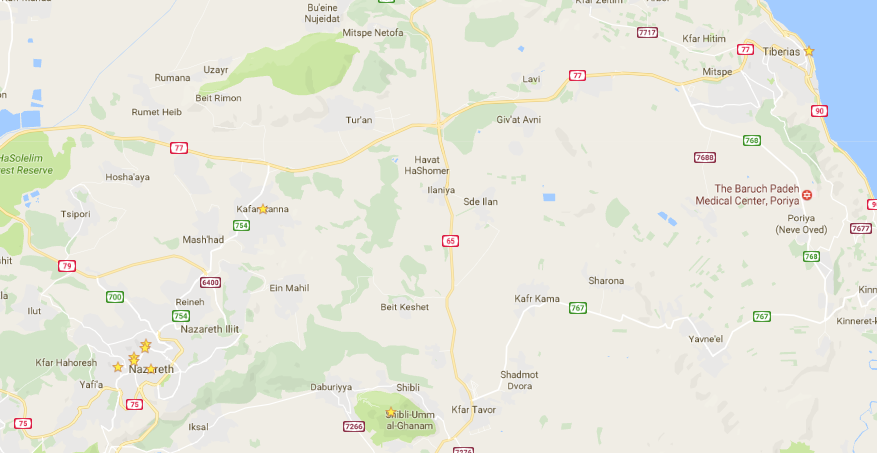
\includegraphics[width=\textwidth]{TiberiasCanaNazarethTabor}

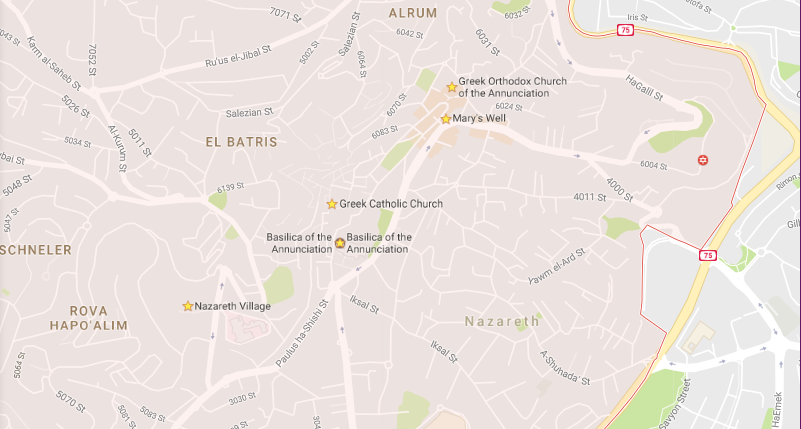
\includegraphics[width=\textwidth]{Nazareth}


\clearpage
\subsection{Cana, the Site of Christ's First Miracle}
\begin{multicols}{2}
	\mbox{}
\end{multicols}
\subsubsection{Scripture}

{\centering
	\emph{\bibleverse{John}(2:1-12) The Wedding at Cana}\\
}
\begin{multicols}{2}
On the third day there was a marriage at Cana in Galilee, and the mother of Jesus was there; 2 Jesus also was invited to the marriage, with his disciples. 3 When the wine gave out, the mother of Jesus said to him, “They have no wine.” 4 And Jesus said to her, “O woman, what have you to do with me? My hour has not yet come.” 5 His mother said to the servants, “Do whatever he tells you.” 6 Now six stone jars were standing there, for the Jewish rites of purification, each holding twenty or thirty gallons. 7 Jesus said to them, “Fill the jars with water.” And they filled them up to the brim. 8 He said to them, “Now draw some out, and take it to the steward of the feast.” So they took it. 9 When the steward of the feast tasted the water now become wine, and did not know where it came from (though the servants who had drawn the water knew), the steward of the feast called the bridegroom 10 and said to him, “Every man serves the good wine first; and when men have drunk freely, then the poor wine; but you have kept the good wine until now.” 11 This, the first of his signs, Jesus did at Cana in Galilee, and manifested his glory; and his disciples believed in him.

12 After this he went down to Caper′na-um, with his mother and his brothers and his disciples; and there they stayed for a few days.
\end{multicols}

\clearpage
\subsection{Site of the Annunciation}
\begin{multicols}{2}
	\mbox{}
\end{multicols}
\subsubsection{Scripture}

{\centering
	\emph{\bibleverse{Luke}(1:24-38) The Birth of Jesus Foretold}\\
}
\begin{multicols}{2}
24 After these days his wife Elizabeth conceived, and for five months she hid herself, saying, 25 “Thus the Lord has done to me in the days when he looked on me, to take away my reproach among men.”

26 In the sixth month the angel Gabriel was sent from God to a city of Galilee named Nazareth, 27 to a virgin betrothed to a man whose name was Joseph, of the house of David; and the virgin’s name was Mary. 28 And he came to her and said, “Hail, O favored one, the Lord is with you!” 29 But she was greatly troubled at the saying, and considered in her mind what sort of greeting this might be. 30 And the angel said to her, “Do not be afraid, Mary, for you have found favor with God. 31 And behold, you will conceive in your womb and bear a son, and you shall call his name Jesus.

\begin{verse}
32 He will be great, and will be called the Son of the Most High;\\
and the Lord God will give to him the throne of his father David,\\
33 and he will reign over the house of Jacob for ever;\\
and of his kingdom there will be no end.”\\
\end{verse}

34 And Mary said to the angel, “How shall this be, since I have no husband?” 35 And the angel said to her,

\begin{verse}
“The Holy Spirit will come upon you,\\
and the power of the Most High will overshadow you;\\
therefore the child to be born will be called holy,\\
the Son of God.\\
\end{verse}
36 And behold, your kinswoman Elizabeth in her old age has also conceived a son; and this is the sixth month with her who was called barren. 37 For with God nothing will be impossible.” 38 And Mary said, “Behold, I am the handmaid of the Lord; let it be to me according to your word.” And the angel departed from her.

\end{multicols}

\clearpage
\subsection{ Mount Tabor}
\begin{multicols}{2}
	\mbox{}
\end{multicols}
\subsubsection{Scripture}

{\centering
	\emph{\bibleverse{Luke}(9:28-36) The Transfiguration}\\
}
\begin{multicols}{2}
28 Now about eight days after these sayings he took with him Peter and John and James, and went up on the mountain to pray. 29 And as he was praying, the appearance of his countenance was altered, and his raiment became dazzling white. 30 And behold, two men talked with him, Moses and Eli′jah, 31 who appeared in glory and spoke of his departure, which he was to accomplish at Jerusalem. 32 Now Peter and those who were with him were heavy with sleep, and when they wakened they saw his glory and the two men who stood with him. 33 And as the men were parting from him, Peter said to Jesus, “Master, it is well that we are here; let us make three booths, one for you and one for Moses and one for Eli′jah”—not knowing what he said. 34 As he said this, a cloud came and overshadowed them; and they were afraid as they entered the cloud. 35 And a voice came out of the cloud, saying, “This is my Son, my Chosen;[a] listen to him!” 36 And when the voice had spoken, Jesus was found alone. And they kept silence and told no one in those days anything of what they had seen.
\end{multicols}

{\centering
	\emph{\bibleverse{Matthew}(17:1-9) The Transfiguration}\\
}
\begin{multicols}{2}
And after six days Jesus took with him Peter and James and John his brother, and led them up a high mountain apart. 2 And he was transfigured before them, and his face shone like the sun, and his garments became white as light. 3 And behold, there appeared to them Moses and Eli′jah, talking with him. 4 And Peter said to Jesus, “Lord, it is well that we are here; if you wish, I will make three booths here, one for you and one for Moses and one for Eli′jah.” 5 He was still speaking, when lo, a bright cloud overshadowed them, and a voice from the cloud said, “This is my beloved Son,[a] with whom I am well pleased; listen to him.” 6 When the disciples heard this, they fell on their faces, and were filled with awe. 7 But Jesus came and touched them, saying, “Rise, and have no fear.” 8 And when they lifted up their eyes, they saw no one but Jesus only.

9 And as they were coming down the mountain, Jesus commanded them, “Tell no one the vision, until the Son of man is raised from the dead.”
\end{multicols}

\clearpage
\subsection{Daily Notes}

\clearpage
\subsection{Journal Entry}

%%%%%%%%%%%%%%%%%%%%%%%%%%%%%%%%%%%%%%%%%%%%%%%%%%%%%%%%%%%%%%%%%%%%%%%%%%%%%%%
%%%%%%%%%%%%%%%%%%%%%%%%%%%%%%%%%%%%%%%%%%%%%%%%%%%%%%%%%%%%%%%%%%%%%%%%%%%%%%%
\chapter{Reflections}
%%%%%%%%%%%%%%%%%%%%%%%%%%%%%%%%%%%%%%%%%%%%%%%%%%%%%%%%%%%%%%%%%%%%%%%%%%%%%%%
\section{Feb 1}
Travel Back Day - On the plane and reflecting on it all

\begin{appendix}
	\chapter{Pilgrimage Announcement - Fr. Gregory}
	\clearpage
	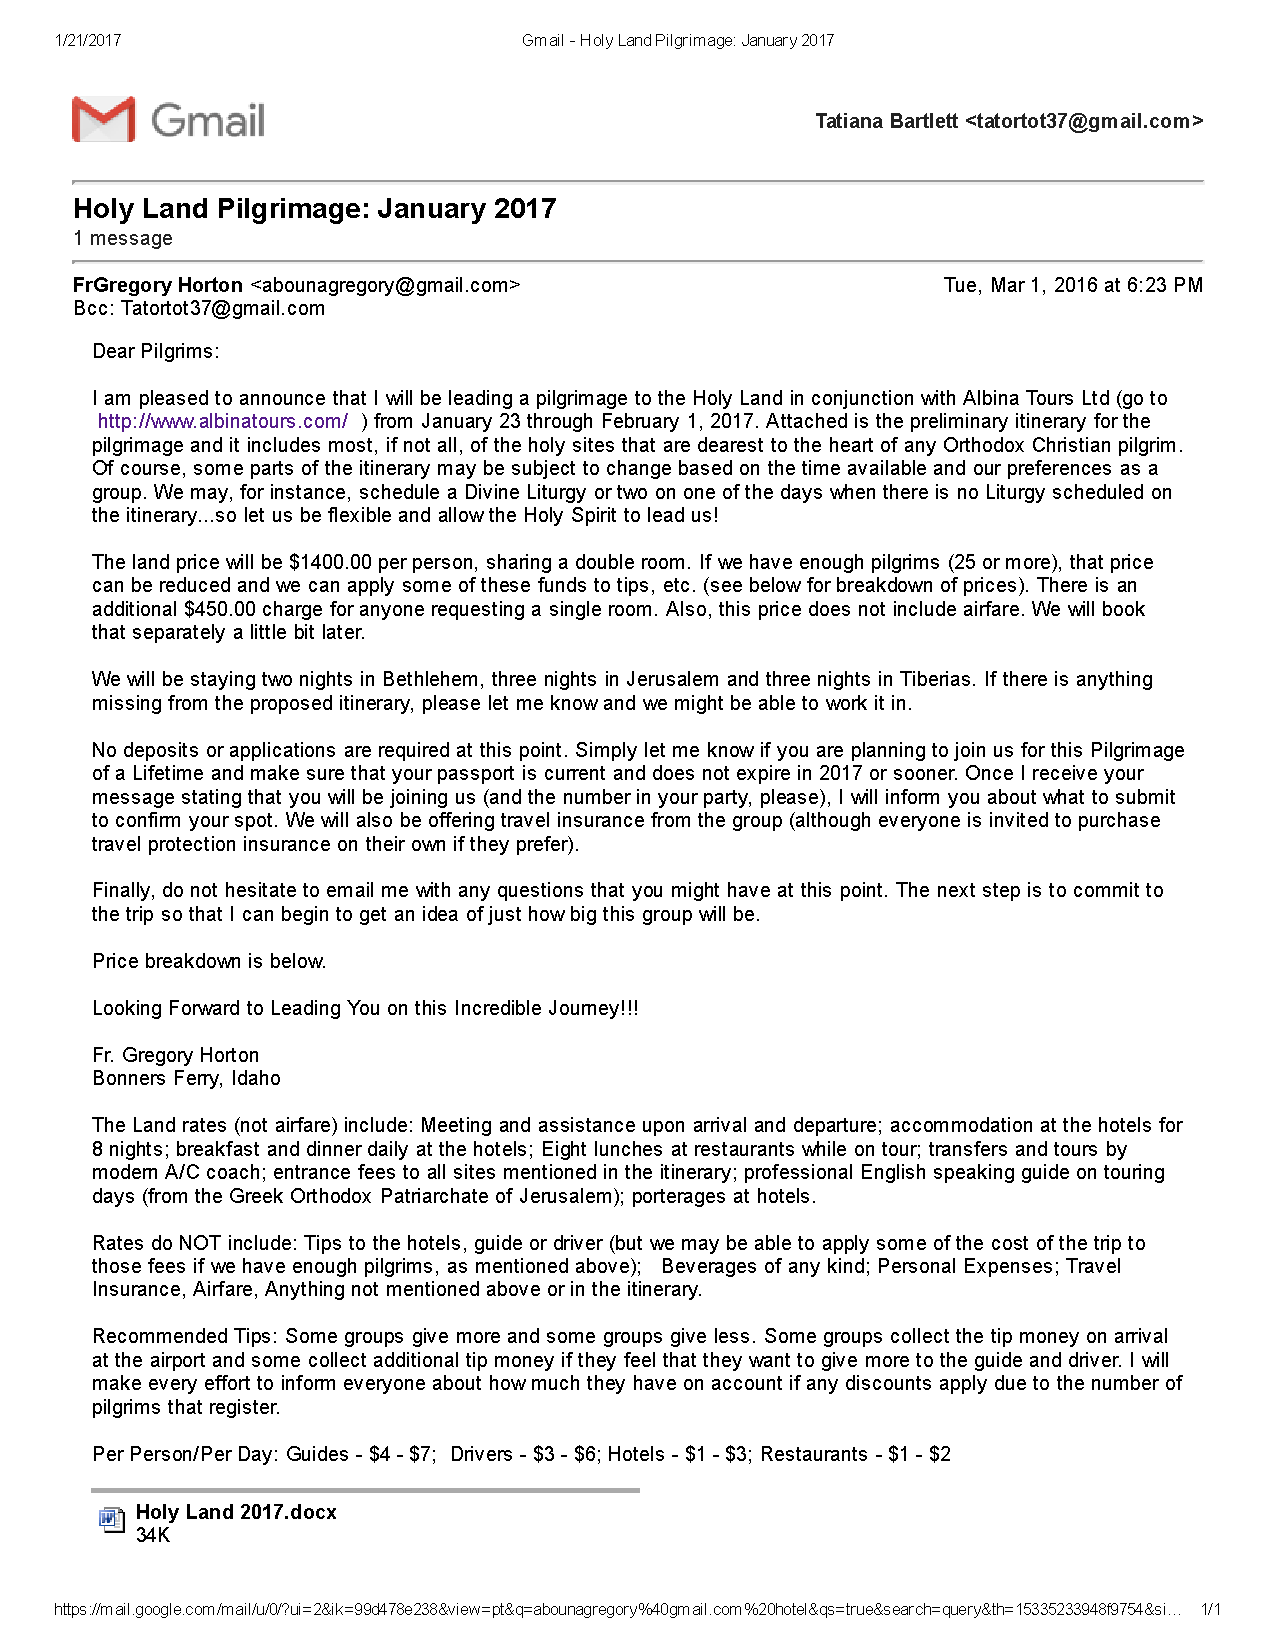
\includepdf[pages=-]{./IsraelAttachments/FrGregoryHolyLandPilgrimage2017}
	\chapter{Albina Tours Ltd}
	\clearpage
	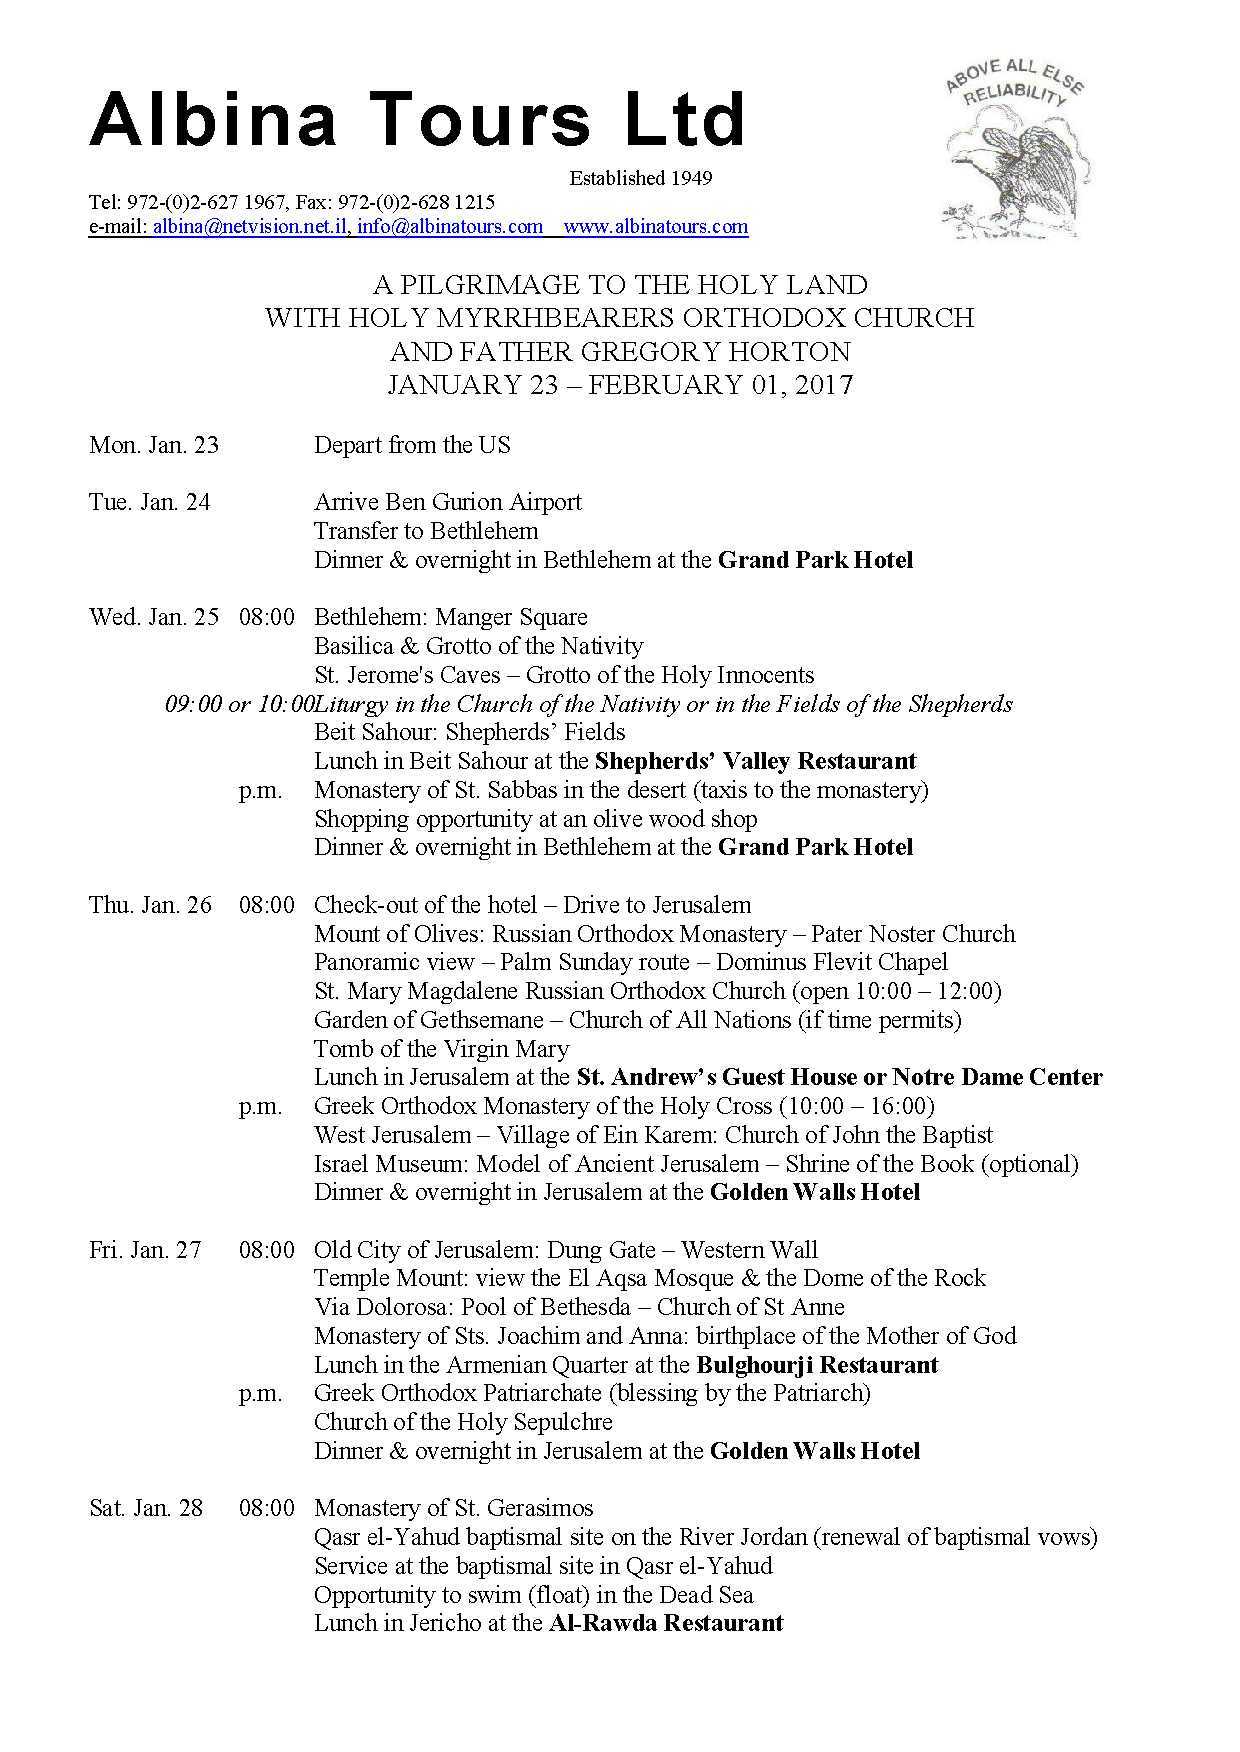
\includepdf[pages=-]{./IsraelAttachments/AlbinaToursLtdPilgrimageIttn}
	\chapter{Plane Tickets}
	\clearpage
	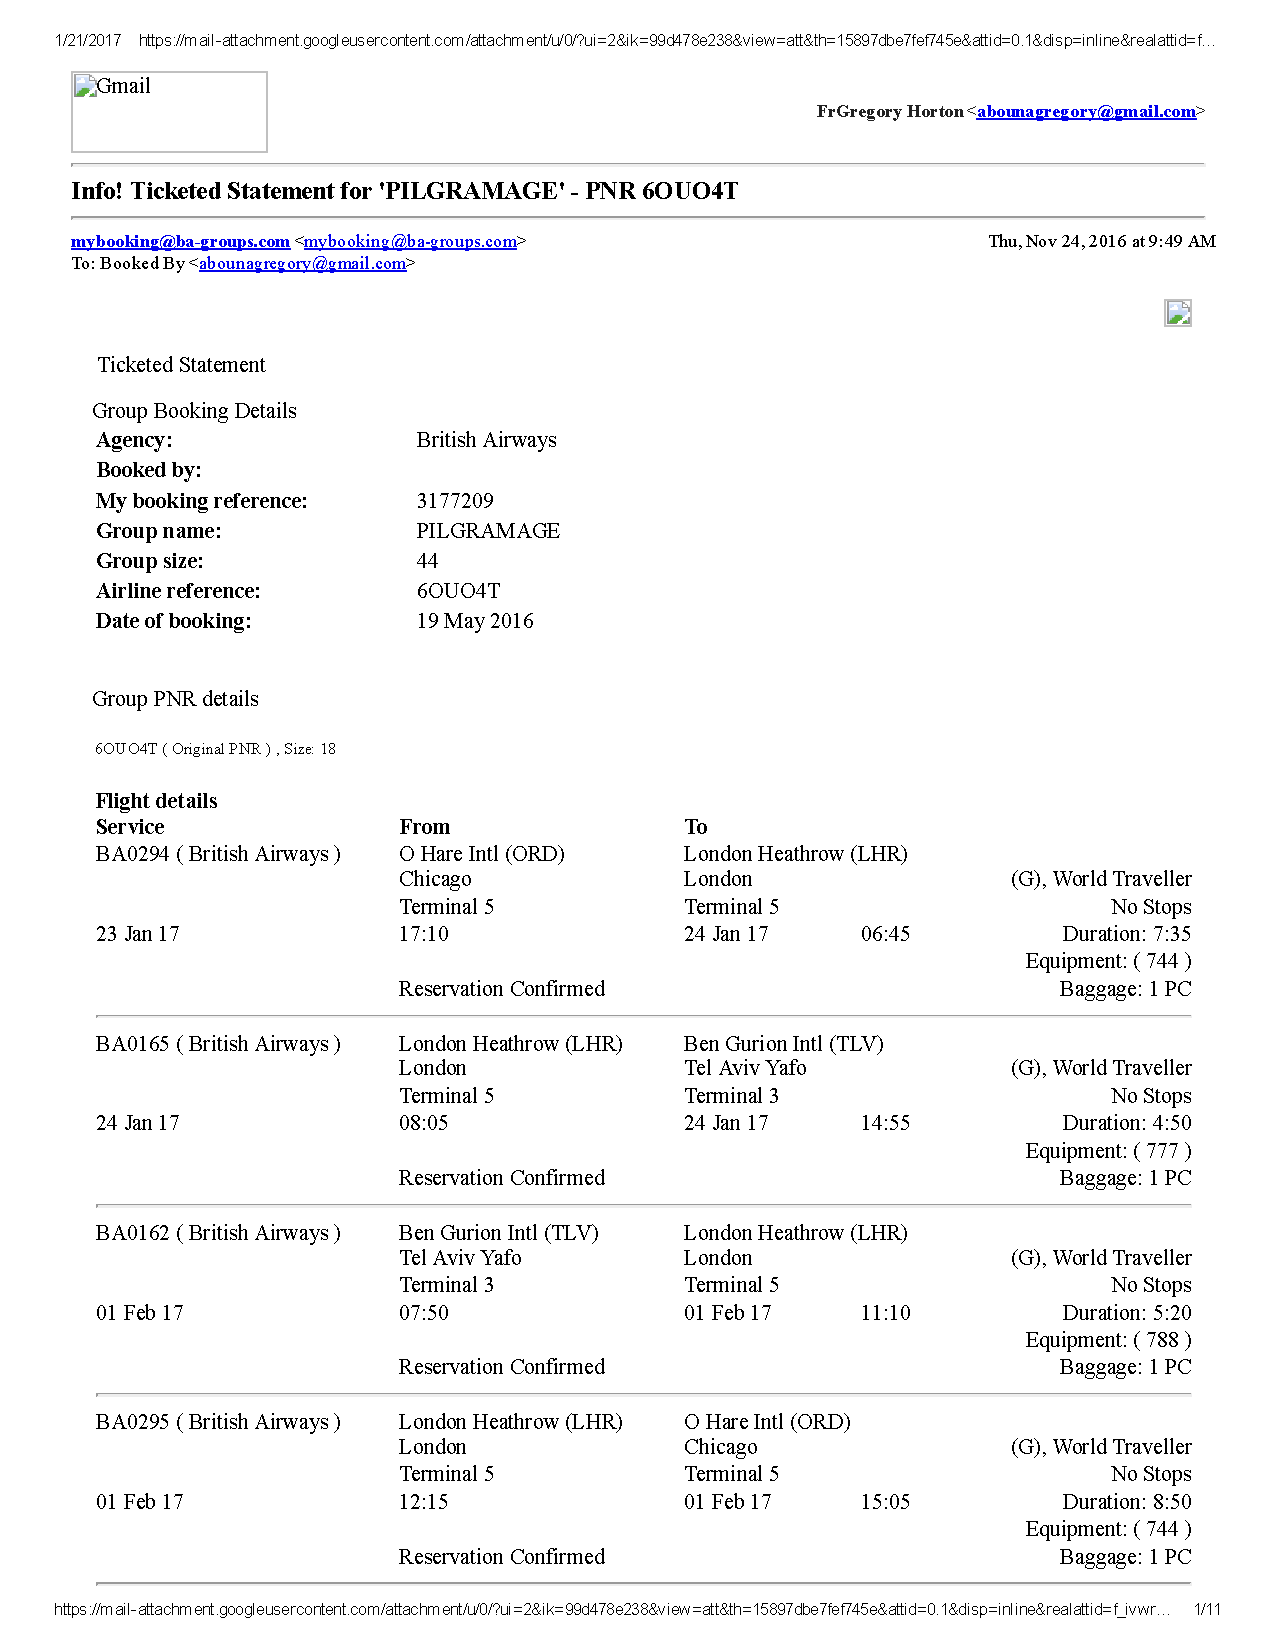
\includepdf[pages=-]{./IsraelAttachments/BookedPlaneIttn}

\end{appendix}

\end{document}
